% Options for packages loaded elsewhere
\PassOptionsToPackage{unicode}{hyperref}
\PassOptionsToPackage{hyphens}{url}
%
\documentclass[
  man,floatsintext]{apa6}
\usepackage{amsmath,amssymb}
\usepackage{lmodern}
\usepackage{iftex}
\ifPDFTeX
  \usepackage[T1]{fontenc}
  \usepackage[utf8]{inputenc}
  \usepackage{textcomp} % provide euro and other symbols
\else % if luatex or xetex
  \usepackage{unicode-math}
  \defaultfontfeatures{Scale=MatchLowercase}
  \defaultfontfeatures[\rmfamily]{Ligatures=TeX,Scale=1}
\fi
% Use upquote if available, for straight quotes in verbatim environments
\IfFileExists{upquote.sty}{\usepackage{upquote}}{}
\IfFileExists{microtype.sty}{% use microtype if available
  \usepackage[]{microtype}
  \UseMicrotypeSet[protrusion]{basicmath} % disable protrusion for tt fonts
}{}
\makeatletter
\@ifundefined{KOMAClassName}{% if non-KOMA class
  \IfFileExists{parskip.sty}{%
    \usepackage{parskip}
  }{% else
    \setlength{\parindent}{0pt}
    \setlength{\parskip}{6pt plus 2pt minus 1pt}}
}{% if KOMA class
  \KOMAoptions{parskip=half}}
\makeatother
\usepackage{xcolor}
\IfFileExists{xurl.sty}{\usepackage{xurl}}{} % add URL line breaks if available
\IfFileExists{bookmark.sty}{\usepackage{bookmark}}{\usepackage{hyperref}}
\hypersetup{
  pdftitle={Assessing sampling methods for generalization from multi-site randomized trials: Modeling recruitment and participation},
  pdfauthor={Gleb Furman1, James E. Pustejovsky2, \& Elizabeth Tipton3},
  pdflang={en-EN},
  pdfkeywords={generalizability, balanced sampling, stratification, multi-site trial},
  hidelinks,
  pdfcreator={LaTeX via pandoc}}
\urlstyle{same} % disable monospaced font for URLs
\usepackage{graphicx}
\makeatletter
\def\maxwidth{\ifdim\Gin@nat@width>\linewidth\linewidth\else\Gin@nat@width\fi}
\def\maxheight{\ifdim\Gin@nat@height>\textheight\textheight\else\Gin@nat@height\fi}
\makeatother
% Scale images if necessary, so that they will not overflow the page
% margins by default, and it is still possible to overwrite the defaults
% using explicit options in \includegraphics[width, height, ...]{}
\setkeys{Gin}{width=\maxwidth,height=\maxheight,keepaspectratio}
% Set default figure placement to htbp
\makeatletter
\def\fps@figure{htbp}
\makeatother
\setlength{\emergencystretch}{3em} % prevent overfull lines
\providecommand{\tightlist}{%
  \setlength{\itemsep}{0pt}\setlength{\parskip}{0pt}}
\setcounter{secnumdepth}{5}
% Make \paragraph and \subparagraph free-standing
\ifx\paragraph\undefined\else
  \let\oldparagraph\paragraph
  \renewcommand{\paragraph}[1]{\oldparagraph{#1}\mbox{}}
\fi
\ifx\subparagraph\undefined\else
  \let\oldsubparagraph\subparagraph
  \renewcommand{\subparagraph}[1]{\oldsubparagraph{#1}\mbox{}}
\fi
\newlength{\cslhangindent}
\setlength{\cslhangindent}{1.5em}
\newlength{\csllabelwidth}
\setlength{\csllabelwidth}{3em}
\newlength{\cslentryspacingunit} % times entry-spacing
\setlength{\cslentryspacingunit}{\parskip}
\newenvironment{CSLReferences}[2] % #1 hanging-ident, #2 entry spacing
 {% don't indent paragraphs
  \setlength{\parindent}{0pt}
  % turn on hanging indent if param 1 is 1
  \ifodd #1
  \let\oldpar\par
  \def\par{\hangindent=\cslhangindent\oldpar}
  \fi
  % set entry spacing
  \setlength{\parskip}{#2\cslentryspacingunit}
 }%
 {}
\usepackage{calc}
\newcommand{\CSLBlock}[1]{#1\hfill\break}
\newcommand{\CSLLeftMargin}[1]{\parbox[t]{\csllabelwidth}{#1}}
\newcommand{\CSLRightInline}[1]{\parbox[t]{\linewidth - \csllabelwidth}{#1}\break}
\newcommand{\CSLIndent}[1]{\hspace{\cslhangindent}#1}
\ifLuaTeX
\usepackage[bidi=basic]{babel}
\else
\usepackage[bidi=default]{babel}
\fi
\babelprovide[main,import]{english}
% get rid of language-specific shorthands (see #6817):
\let\LanguageShortHands\languageshorthands
\def\languageshorthands#1{}
% Manuscript styling
\usepackage{upgreek}
\captionsetup{font=singlespacing,justification=justified}

% Table formatting
\usepackage{longtable}
\usepackage{lscape}
% \usepackage[counterclockwise]{rotating}   % Landscape page setup for large tables
\usepackage{multirow}		% Table styling
\usepackage{tabularx}		% Control Column width
\usepackage[flushleft]{threeparttable}	% Allows for three part tables with a specified notes section
\usepackage{threeparttablex}            % Lets threeparttable work with longtable

% Create new environments so endfloat can handle them
% \newenvironment{ltable}
%   {\begin{landscape}\centering\begin{threeparttable}}
%   {\end{threeparttable}\end{landscape}}
\newenvironment{lltable}{\begin{landscape}\centering\begin{ThreePartTable}}{\end{ThreePartTable}\end{landscape}}

% Enables adjusting longtable caption width to table width
% Solution found at http://golatex.de/longtable-mit-caption-so-breit-wie-die-tabelle-t15767.html
\makeatletter
\newcommand\LastLTentrywidth{1em}
\newlength\longtablewidth
\setlength{\longtablewidth}{1in}
\newcommand{\getlongtablewidth}{\begingroup \ifcsname LT@\roman{LT@tables}\endcsname \global\longtablewidth=0pt \renewcommand{\LT@entry}[2]{\global\advance\longtablewidth by ##2\relax\gdef\LastLTentrywidth{##2}}\@nameuse{LT@\roman{LT@tables}} \fi \endgroup}

% \setlength{\parindent}{0.5in}
% \setlength{\parskip}{0pt plus 0pt minus 0pt}

% Overwrite redefinition of paragraph and subparagraph by the default LaTeX template
% See https://github.com/crsh/papaja/issues/292
\makeatletter
\renewcommand{\paragraph}{\@startsection{paragraph}{4}{\parindent}%
  {0\baselineskip \@plus 0.2ex \@minus 0.2ex}%
  {-1em}%
  {\normalfont\normalsize\bfseries\itshape\typesectitle}}

\renewcommand{\subparagraph}[1]{\@startsection{subparagraph}{5}{1em}%
  {0\baselineskip \@plus 0.2ex \@minus 0.2ex}%
  {-\z@\relax}%
  {\normalfont\normalsize\itshape\hspace{\parindent}{#1}\textit{\addperi}}{\relax}}
\makeatother

% \usepackage{etoolbox}
\makeatletter
\patchcmd{\HyOrg@maketitle}
  {\section{\normalfont\normalsize\abstractname}}
  {\section*{\normalfont\normalsize\abstractname}}
  {}{\typeout{Failed to patch abstract.}}
\patchcmd{\HyOrg@maketitle}
  {\section{\protect\normalfont{\@title}}}
  {\section*{\protect\normalfont{\@title}}}
  {}{\typeout{Failed to patch title.}}
\makeatother

\usepackage{xpatch}
\makeatletter
\xapptocmd\appendix
  {\xapptocmd\section
    {\addcontentsline{toc}{section}{\appendixname\ifoneappendix\else~\theappendix\fi\\: #1}}
    {}{\InnerPatchFailed}%
  }
{}{\PatchFailed}
\keywords{generalizability, balanced sampling, stratification, multi-site trial}
\usepackage{csquotes}
\usepackage{rotating}
\usepackage{float}
\geometry{twoside=false, top=1in, bottom=1in, left=1in, right=1.15in}
\usepackage[textwidth=1in, textsize=tiny]{todonotes}
\raggedbottom
\newcommand{\JEP}[1]{\todo[color=blue!20]{#1}}
\newcommand{\GF}[1]{\todo[color=orange]{#1}}
\ifLuaTeX
  \usepackage{selnolig}  % disable illegal ligatures
\fi

\title{Assessing sampling methods for generalization from multi-site randomized trials: Modeling recruitment and participation}
\author{Gleb Furman\textsuperscript{1}, James E. Pustejovsky\textsuperscript{2}, \& Elizabeth Tipton\textsuperscript{3}}
\date{}


\shorttitle{Assessing sampling methods for generalization from MRTs}

\authornote{

Correspondence concerning this article should be addressed to Gleb Furman, University of Texas at Austin, SZB 504, 1912 Speedway, Austin, Texas 78712. E-mail: \href{mailto:gleb.furman@utexas.edu}{\nolinkurl{gleb.furman@utexas.edu}}

}

\affiliation{\vspace{0.5cm}\textsuperscript{1} University of Texas at Austin\\\textsuperscript{2} University of Wisconsin-Madison\\\textsuperscript{3} Northwestern University}

\abstract{%
In the ideal, educational research aimed at informing policy decisions should support causal inferences at the population level. However, large scale, multi-site randomized trials often rely on convenience sampling methodology when recruiting districts and schools, resulting in relatively homogeneous samples that may differ systematically from the intended population of interest. Designing sampling methods that focus on generalizability may be a more effective approach. However, there is a lack of methodological research examining the effectiveness of such strategies in education research contexts. We describe a framework for conducting such methodological evaluations based on formal models for study recruitment and participation. Using this framework, we examine one promising method, stratified balanced sampling (SBS), in the context of recruiting a representative sample of schools for a large trial. Using simulations based on a realistic sampling frame, we compare SBS to stratified and unstratified versions of convenience sampling and probability sampling. Under our modeling assumptions, we find that SBS and stratified random sampling result in highly generalizable samples. However, implementing these methods requires extensive recruitment efforts when willingness to participate is low. Stratified convenience sampling represents a potential compromise. Further empirical research into recruitment and participation behavior is needed to better evaluate sampling methods under realistic conditions.
}



\begin{document}
\maketitle

\hypertarget{sampling-for-generalization}{%
\section*{Sampling for generalization}\label{sampling-for-generalization}}
\addcontentsline{toc}{section}{Sampling for generalization}

The multi-site randomized trial has become a more common design for evaluating the effects of educational interventions. An multi-site randomized trial is a randomized experiment that takes place across multiple distinct sites, such as school districts, medical clinics, or geographic areas, with random assignment taking place either at the unit level (i.e., blocked randomization by site) or site level (i.e., cluster randomization). In education research, a multi-site trial might entail recruiting multiple schools in each of several districts. Once a sample of schools is recruited, students, classes, teachers, or whole schools are randomly assigned either to receive an intervention (treatment group) or to an alternative condition, such as continuing business-as-usual (control group).

Well-executed multi-site trials with low attrition support a high level of internal validity, in that one can be confident that observed differences in outcomes between the treatment and control groups represent causal effects of treatment assignment for the sample of participating units. One might also expect that running a trial across multiple sites would support a high level of external validity, or generalizability, because it provides a basis for detecting and investigating cross-site variation in treatment effects (Raudenbush \& Bloom, 2015). Compared to using a single-site design, running an experiment across multiple sites allows researchers to generalize findings to a larger population of sites if the participating sites can be intepreted as a representative sample from that population (Raudenbush \& Liu, 2000). However, such claims of generalizability rest on strong and rather ambiguous assumptions about the goal of generalization.

In the context of intervention studies, generalizability describes how well the effect of an intervention would hold for units outside of the study. For instance, results of a randomized trial are often interpreted as estimates of the sample average treatment effect (SATE), or the average effect of intervention for the set of units that actually participated in the study (Gerber \& Green, 2012). If the study sample is representative of a larger population, a SATE estimate can also be interpreted as a reasonable estimate of the average effect of intervention within the larger population of units, or population average treatment effect (PATE), without any additional adjustments. However, if the sample is compositionally different from the population of interest, and if response to intervention varies across units or sites in the population, then the SATE no longer provides an unbiased estimate of the PATE (Imai, King, \& Stuart, 2008).

Several studies have found that schools and districts that participate in large scale randomized trials differ substantially from the national population and from policy-relevant sub-populations (Fellers, 2017; Stuart, Bell, Ebnesajjad, Olsen, \& Orr, 2017; Tipton, Spybrook, Fitzgerald, Wang, \& Davidson, 2020). This suggests that current research practices yield non-representative samples. In turn, non-representative samples may lead to substantially biased estimates of population-level effects (Olsen, Orr, Bell, \& Stuart, 2013; Shadish, Cook, \& Campbell, 2002). Beyond accurate effects estimates, lack of representation in multi-site trials can also be a question of equity. For instance, small under-served rural districts are under-represented in randomized trials sponsored by Institute of Education Sciences (Fellers, 2017; Stuart et al., 2017; Tipton et al., 2020), and thus may be less likely to benefit from federally funded education research.

One way to achieve strong generalizability is to select sites from a well-defined population using known probabilities of selection. If the design uses random assignment and attains high compliance and low attrition, it enables unbiased estimation of the SATE. Using the known sampling probabilities, the SATE can then be adjusted to estimate the PATE. Unfortunately, probability sampling is rarely used in large-scale impact evaluations (Olsen et al., 2013; Shadish et al., 2002). Instead, researchers often opt for convenience or purposive sampling. These methods are much less expensive to implement, but are not usually designed to achieve population representation.

\hypertarget{retrospective-generalization-methods}{%
\subsection*{Retrospective generalization methods}\label{retrospective-generalization-methods}}
\addcontentsline{toc}{subsection}{Retrospective generalization methods}

A growing body of methodological research has considered how to estimate PATEs from non-representative samples using retrospective propensity score analysis (Kern, Stuart, Hill, \& Green, 2016; O'Muircheartaigh \& Hedges, 2014; Stuart, Cole, Bradshaw, \& Leaf, 2011; Tipton, 2013). Estimation entails re-weighing the sample or making model-based statistical adjustments to represent a population of interest.
These methods rely on the availability of data clearly defining the inference population in order to justify a claim of generalizability. Specifically, data must enumerate all units in the population and include information on characteristics of the units that predict treatment effect heterogeneity. These requirements make retrospective methods especially salient in randomized trials of educational interventions due to the availability of extensive data on districts and schools (e.g., the Common Core of Data, the Stanford Education Data Archive, etc.).

A shortcoming of retrospective generalization methods is under-coverage (Chan, 2017; Groves, 2004) which occurs when a sample lacks units corresponding to a sub-group of the inference population. Under-coverage can be assessed using several techniques that identify how well a sample would generalize to a specific population (Stuart et al., 2011; Tipton, 2014a). If under-coverage is great enough to prevent use of statistical adjustment for estimating the PATE, then the inference population must be redefined. However, re-defining the inference population diminishes the relevance of study results, undermining the benefits of large-scale multi-site trials.

\hypertarget{stratified-balanced-sampling}{%
\subsection*{Stratified balanced sampling}\label{stratified-balanced-sampling}}
\addcontentsline{toc}{subsection}{Stratified balanced sampling}

Rather than relying solely on retrospective adjustments, researchers can also address generalizability during the design and recruitment stages of a study, using robust sampling methods to obtain more representative samples (Tipton, 2013, 2014b). Like retrospective adjustment, these methods also require extant data on a well-defined and enumerated population.
One method in particular, Stratified Balanced Sampling (SBS), has received attention from intervention effectiveness researchers due to its accessibility and relevance to trials of educational interventions (Tipton \& Olsen, 2018).

SBS involves using cluster analysis to split the population into smaller, more homogeneous strata. Sites within each stratum are ranked according to how well they represent the stratum and highly representative sites are prioritized for recruitment.
Researchers who are interested in using this approach to sample schools may even use a website (www.thegeneralizer.org) that guides them through the process using a sampling frame from the Common Core of Data.

Several studies have described potential theoretical benefits of SBS (Tipton, 2014b; Tipton et al., 2016). First, SBS requires that researchers specify the inference population and justify targeting specific sites. Thus, it enforces a degree of clarity regarding the goal of generalization, which has often been lacking even in large-scale multi-site trials in education (Tipton et al., 2020). Second, SBS should theoretically improve sample representation and reduce under-coverage, thereby improving generalization to the specified target population. Further, SBS easily integrates with retrospective statistical adjustment techniques. Even if balance is only partially improved at the sampling stage, coverage errors should still be reduced, mitigating the need to redefine the inference population post-hoc.
Finally, SBS requires researchers to carefully document the recruitment process, which supports transparency and enables more rigorous critique of the sampling design and study inferences, as well as enabling follow-up analysis on participation behavior such as systematic differences between participants and non-responders.

SBS is also limited in several respects. The method depends on the existence of a rich set of observed covariates related to treatment heterogeneity and sample selection for each site in the population. Readily available extant data consist primarily of demographics and may not contain information on covariates that are more proximally related to variation in treatment effects, which can result in omitted variable bias (Tipton, 2014b). Additionally, implementing SBS may require more resources than a simple convenience sample because recruiting ranked sites from multiple strata requires a coordinated effort between recruiters (Tipton, Hallberg, Hedges, \& Chan, 2017; Tipton \& Matlen, 2019). This means that recruiters cannot work independently and must work in coordination with methodologists to implement the sampling strategy.

At least one research group has implemented SBS in a large-scale multi-site educational intervention study and documented their experiences (Tipton \& Matlen, 2019). The authors reported success in selecting a highly generalizable sample, but substantial efforts were required to develop the sample frame, generate optimal strata, and coordinate with recruiters.
This was compounded by the unavailability of data necessary for identifying the sampling frame.
Additionally, though the recruiters reported that working within the strata did not burden their efforts, certain strata were more difficult to recruit from than others.
These findings raise an important and pragmatic question: do the advantages of SBS justify the additional resources necessary to implement it?
And how do other methods of sample recruitment compare in terms of their ability to obtain representative samples and their cost to implement?

\hypertarget{aims}{%
\subsection*{Aims}\label{aims}}
\addcontentsline{toc}{subsection}{Aims}

In order for researchers to make informed decisions about sampling strategies, there is a need to better understand both the performance and the cost of SBS in comparison to other sample recruitment methods.
The goal of the current paper is to describe a framework for making such assessments and to demonstrate how it can be applied.
Central to our proposed framework is that sample representation is influenced by two distinct processes: the researcher's recruitment method and schools' participation decisions.
The recruitment method influences whether a site is approached by researchers; possible methods include SBS, probability sampling, and convenience sampling.
Because convenience sampling can take many forms in practice, we sketch a simple model prioritizing sites that are more likely to agree to participate.
The second process involves site participation decisions.
To model these decisions, we use extant demographic data and reported characteristics of schools that have been recruited to large-scale trials to simulate a participation propensity score.

After describing formal models for recruitment and participation, we report a simulation study comparing the generalizability and feasibility of the sampling methods. We conceptualize generalizability in terms of whether obtained samples are similar to the target population on observable site characteristics. We conceptualize
feasibility in terms of researcher recruitment effort to obtain a target sample size and how sample participation is distributed across the population.
As with many simulation studies, findings from those reported below are tentative and limited due to some of the simplifying assumptions that we impose--particularly assumptions about the site participation model and the process of convenience sampling.
Despite these assumptions, we argue that the simulations nonetheless provide insights into the relative performance of different recruitment methods.
Moreover, the limitations of the simulations also highlight current the need for better empirical data about recruitment efforts, so that key assumptions of the framework can be further refined.

The remainder of the paper is organized as follows. In the next section, we describe the framework for assessing recruitment methods by proposing a model for site participation decisions and several models for sample recruitment, including SBS and other sampling methods.
We then demonstrate how to implement our proposed framework in a simulation, in which we assess the relative performance of SBS and other recruitment methods. In the final two sections, we report the simulation results and discuss limitations and directions for future research in this area.

\hypertarget{methods-and-models}{%
\section*{Methods and Models}\label{methods-and-models}}
\addcontentsline{toc}{section}{Methods and Models}

The goal of recruitment is to obtain a study sample that is compositionally similar to a population of interest, such that treatment effects detected in the study can be generalized to that population.
Ideally, we would like to obtain a sample that is similar to the population on any and all characteristics that are related to treatment effect heterogeneity.
However, both SBS and retrospective generalization methods have a more conscribed goal, seeking generalizability with respect to measured variables in the sampling frame, such as school demographics (e.g.~ethnic composition, urbanicity) or general academic achievement information (e.g., performance on standardized tests in math or English Language Arts).
We will follow the latter conceptualization of generalizability.

Formally, we consider a population of \(N\) units (such as schools), indexed by \(j = 1,...,N\).
We assume that we have a data set containing \(P\) covariates, \(\mathbf{x}_j = \left(x_{1j},...,x_{Pj}\right)\), for every unit in the population. The covariates may be a mixture of continuous, binary, and categorical data.
Following Tipton (2014b), we assume that the researcher's goal is to select a sample of \(n\) sites such that there is balance along \(\mathbf{x}_j\) between the sample and the population, indicating that the population is compositionally represented by the sample.
We measure balance using the standardized mean difference (\(SMD\)) between the sample and population for a given covariate. For covariate \(p\), the SMD is calculated as
\begin{align} \label{eq:SMD}
SMD_p = \frac{\bar{x}_p - \mu_p}{\sigma_p}
\end{align}
where \(\bar{x}_p\) is the sample mean of covariate \(p\), \(\mu_p\) is the covariate mean in the population, and \(\sigma_p\) is the standard deviation of the covariate in the population. \(SMD\) values closer to zero indicate greater balance between the sample and the population. By this measure, obtaining a \(SMD_p \le 0.25\) for all covariates in \(P\) would indicate that the sample is well balanced and can be generalized to the population. Covariates for which \(SMD_p > 0.25\) would likely require additional statistical adjustment in the final analysis.\todo[color=blue!20]{Citations for these conventions?}

When recruiting a sample, selection bias---or imbalance between the sample and the population---can arise from at least two distinct sources: recruitment methods and the decisions of individual units about whether to participate. Our goal is to assess the effectiveness and costs of different recruitment methods, such as SBS, probability sampling, and convenience sampling. However, any of these recruitment methods must contend with non-response, such as when school leaders decline to participate in the research study.
We model these two processes separately, allowing us to isolate the influence of different recruitment methods.

Formally, let \(P_j\) be an indicator for whether site \(j\) participates in the study. Let \(Z_j\) be an indicator for whether site \(j\) is recruited, or invited to participate in the study. Let \(E_j\) be an indicator for whether site \(j\) agrees to participate, if recruited. In order for site \(j\) to participate, it must both be recruited and agree; it follows that \(P_j = Z_j \times E_j\). For a site with covariates \(\mathbf{x}_j\), the probability of participating in a trial is therefore
\begin{equation}
\label{eq:PZEX}
\Pr\left(P_j = 1 | \mathbf{x}_j \right) = \Pr\left(E_j = 1 | Z_j = 1, \mathbf{x}_j \right) \times \Pr\left(Z_j = 1 | \mathbf{x}_j \right).
\end{equation}
Non-representative samples can result from bias in the recruitment process, which determines \(\Pr\left(Z_j = 1 | \mathbf{x}_j \right)\), from bias in the response process, which determines \(\Pr\left(E_j = 1 | Z_j = 1, \mathbf{x}_j \right)\), or from the interaction of the two.
In the remainder of this section, we introduce formal models for each component process.

\hypertarget{modeling-response-bias}{%
\subsection*{Modeling Response Bias}\label{modeling-response-bias}}
\addcontentsline{toc}{subsection}{Modeling Response Bias}

To describe unit participation decisions (i.e., self-selection), we propose a response propensity score model that involves several key assumptions.
First, we assume that each individual site is responsible for deciding whether to participate, and that site decisions are independent.
That is to say, districts, administrators, teachers, research coordinators, etc., as individual units do not influence decision.
Second, we assume that sites' response decisions are related to their measured covariates, \(\mathbf{x}_j\). Specifically, the decision to participate may be associated with site-level characteristics (e.g., urbanicity, school size) or aggregated student data (e.g., average student demographics, percent of students with IEPs).
Third, we assume that response decisions are not influenced by the recruitment process itself, so that
\begin{equation}
\label{eq:potential-participation}
\Pr\left(E_j = 1 | Z_j = 1, \mathbf{x}_j \right) = \Pr\left(E_j = 1 | \mathbf{x}_j \right).
\end{equation}
Under this assumption, \(E_j\) can be interpreted as an indicator for \emph{potential response}, or whether a site would participate in the study \emph{if approached for recruitment}, for any site in the population.
This simplifying assumption could fail to hold if the likelihood that a site responds depends on the manner of recruitment.\footnote{For example, a school site be more likely to respond to a recruitment attempt made through a face-to-face meeting than one from an email blast.}

Let \(\pi_j\) represent the potential response propensity score, or the probability that site \(j\) agrees to participate in the study if approached for recruitment. We model the potential response propensity using the logistic regression
\begin{align}
\label{eq:RGM}
\log\left(\frac{\pi_j}{1 - \pi_j}\right) = \beta_0 + \mathbf{x}_j \boldsymbol\beta
\end{align}
where \(\mathbf{x}_j\) are covariates that predict sample selection for each unit and \(\boldsymbol\beta\) is a vector of coefficients associated with those covariates. Participation for unit \(j\) is then determined by sampling from a Bernoulli distribution with probability equal to \(\pi_j\):
\begin{equation}
\label{eq:Ej}
E_j \sim B(\pi_j).
\end{equation}
Under this model, \(\pi_j\) is a constant site characteristic, whereas \(E_j\) can vary across replications of the sampling process.

These assumptions are clearly a stylized, and perhaps over-simplified, representation of a complicated and multifaceted decision-making process.
We know, for instance, that in many cases districts act as gatekeepers by determining whether or not to approve research proposals.
However, a more nuanced model may not necessarily be more accurate.
Our understanding of school participation is limited to anecdotal evidence and studies that report sample characteristics.
In the case of the latter, these characteristics themselves are biased as they are subject to the recruitment strategy employed by the researcher. For instance, if a study employed some form of non-probability sampling, differences between that sample and its' intended inference population could be attributed to an unknowable conflation of the recruitment method and non-response.
In the absence of more concrete information about self selection, we believe that the model as proposed is a useful initial representation of what drives schools to participate in evaluations of educational interventions.
While our results will not support inferences about these behaviors, they will nevertheless allow us to compare the performance of sampling methods and how they handle realistic challenges such as non-response.

\hypertarget{sampling-methods}{%
\subsection*{Sampling Methods}\label{sampling-methods}}
\addcontentsline{toc}{subsection}{Sampling Methods}

We now propose formal models for several sampling procedures. The scope of procedures that we review here is not meant to be comprehensive. However, by formalizing them in this fashion we hope to make the procedures transparent, reproducible, and adaptable to other circumstances that researchers may encounter.
For each method, we model the sampling process as observing the potential participation indicator for sites in a ranked list, where the order in which sites are contacted is determined by a score \(S = \{S_1,...,S_N\}\). Different sampling procedures are defined by different methods of determining the scores. Thus, the recruitment indicators \(Z_1,...,Z_N\) are a function of the scores, \(Z_j = Z_j(S)\) for \(j = 1,...,N\).
For the un-stratified sampling methods, we determined \(Z_1(S),...,Z_N(S)\) by sorting sites according to \(S\) and selecting the first \(n\) sites with \(E_j = 1\).
Specifically,
\begin{equation}
\label{eq:Zj}
Z_j(S) = I\left[n \geq \sum_{i=1}^N E_i I\left(S_i \leq S_j\right)\right]
\end{equation}
where \(I(C)\) denotes the indicator function, equal to 1 if \(C\) is true and otherwise equal to 0. Based on the sample selection indicators, we calculate the number of sites contacted as
\begin{equation}
\label{eq:R}
R(S) =  \max \{S_1 Z_1, S_2 Z_2, ..., S_N Z_N\}.
\end{equation}
This model is again a stylized representation of a real recruitment process, but still one that we think is useful to study.\footnote{In practice, recruitment occurs over time and recruiters may be in contact with multiple potential sites at any one time (Tipton \& Matlen, 2019). This would suggest that the total number of contacts in a real recruitment process might exceed \(R(S)\).}

Stratified sampling gives researchers more control over the characteristics of their sample. Consider the case of random sampling, which only produces a representative sample on average. To reduce the likelihood of an ``unlucky'' sample, a population can be split into strata based on characteristics specified by the researcher. Random sampling from within each of the strata will then ensure that each of those characteristics are represented in the final sample. Stratification is routinely used with probability or non-probability sampling methods in survey research.

To model stratified sampling methods, we will assume that the population is divided into a set of \(K\) strata. Proportional allocation will be used to ensure the relative size of the strata in the sample reflects that of the population (Tipton, 2014b).
Letting \(N_k\) denote the total number of sites in stratum \(k\), we set a target sample size of \(n_k = [n \times N_k / N]\) for stratum \(k = 1,...,K\), where \([x]\) is the integer nearest to \(x\).
Let \(G_j \in \{1,...,K\}\) be the stratum assignment of unit \(j\), for \(j = 1,...,N\).
For the stratified sampling methods, the process for determining participation is applied separately within each stratum, so that
\begin{equation}
\label{eq:Zj-strat}
Z_j(S) = I\left[n^{G_j} \geq \sum_{i=1}^N E_i I\left(S_i \leq S_j, G_i = G_j\right)\right]
\end{equation}
and
\begin{equation}
\label{eq:R-strat}
R_k(S) = \max \{S_1 Z_1 I(G_1 = k), ..., S_N Z_N I(G_N = k)\},
\end{equation}
with \(R(S) = \sum_{k=1}^K R_k(S)\).

\hypertarget{random-sampling}{%
\subsection*{Random Sampling}\label{random-sampling}}
\addcontentsline{toc}{subsection}{Random Sampling}

As we previously noted, probability sampling is typically impractical in the context of multi-site randomized trials of educational interventions. However, probability sampling methods are nonetheless interesting as a simple, theoretical ideal against which to compare other sampling methods.
In particular, using probability sampling eliminates recruitment bias, so that any remaining selection bias is due entirely to sites' participation decisions (i.e., non-response bias).
We can simulate unstratified random sampling (URS) by ranking each site at random, so that their order of recruitment \(S\) is determined by sampling without replacement from the integers \(1,...,N\). In practice, methods such as cluster sampling, stratified sampling, or a combination of both would likely offer advantages over unstratified random sampling. We therefore also consider stratified random sampling (SRS), with strata defined by a cluster analysis and using a proportional allocation. For URS, \(\Pr\left(Z_j = 1 | \mathbf{x}_j \right)\) is constant for all \(j = 1,...,N\); for SRS, \(\Pr\left(Z_j = 1 | \mathbf{x}_j \right)\) is constant within each stratum but can vary between strata due to differences in stratum size and average response rates.

\hypertarget{convenience-sampling}{%
\subsection*{Convenience Sampling}\label{convenience-sampling}}
\addcontentsline{toc}{subsection}{Convenience Sampling}

Some form of convenience sampling is probably the most common approach to sample recruitment.
However, researchers rarely operationalize or report their process for selecting a convenience sample, leaving open the questions of what drives recruitment bias and how to model it. As an initial model, we posit that the purpose of convenience sampling is to reduce recruitment effort. If we further assume that recruiters have some prior knowledge (based on field experience) of how likely site are to participate if approached, then we can model convenience sampling as prioritizing sites with a higher propensity to participate. We refer to this as the ``low hanging fruit'' approach to convenience sampling.

As with probability sampling, we will consider two forms of convenience sampling: unstratified and stratified convenience sampling. To operationalize unstratified convenience sampling (UCS), we assume that sites are approached for recruitment one at a time, with their order determined by sampling without replacement, and with probability proportional to the ranks of participation propensity scores. Once a sites is selected and assigned a rank, the next sites is selected with a probability proportional to the weights of the remaining sites. Once all ranks are assigned, sites are approached until \(n\) sites agreed to be in the sample. Let \(\eta_j\) be the integer rank of \(\pi_j\) within the distribution of participation propensity scores \(\pi_1,...,\pi_N\). Then, for UCS,
\begin{equation}
\Pr\left(Z_j = 1 | \mathbf{x}_j \right) = c \eta_j
\end{equation}
for a scaling constant \(c\).
Under this model of convenience sampling, the site with the highest response propensity is twice as likely to be sampled as the site with the median response propensity; the site at the 80th percentile is twice as likely to be sampled as the site at the 40th percentile; etc.
Because they depend only on the ranks of the response propensities, the sampling probabilities will remain the same for location shifts and scale shifts in the distribution of response propensities.
This property allows us to manipulate the parameters of the response propensity model (Equation \eqref{eq:RGM}) without altering the behavior of the convenience sampling process.

We operationalize stratified convenience sampling (SCS) using the same process as for UCS, but with ranks determined independently within each stratum, and using a proportional allocation across strata.

\hypertarget{balanced-sampling}{%
\subsection*{Balanced Sampling}\label{balanced-sampling}}
\addcontentsline{toc}{subsection}{Balanced Sampling}

SBS entails first stratifying the population, then selecting units so that the sample from each stratum matches the corresponding sub-population on a set of covariates. Let \(\mu_{p k}\) denote the mean of covariate \(p\) in population stratum \(k\), for \(p = 1,...,P\) and \(k = 1,...,K\). Given a set of strata, SBS is designed to select units so that
\begin{align}
\frac{1}{n_k} \sum_{j=1}^N X_{pj} \times I\left(Z_j = 1, G_j = k\right) - \mu_{p k},
\end{align}
is small in absolute value for all \(k = 1,...,K\) and \(p = 1,...,P\).

Following Tipton (2014b), we operationalize balanced sampling by generating ranks that prioritize the recruitment of sites based on their similarity to the ``average'' site in each stratum.
Specifically, we ranked each site within a stratum using a weighted Euclidean distance measure, with sites closer to the center of the strata ranked higher. The scores for SBS are thus:
\begin{align} \label{eq:euclid}
S_j = \sqrt{\sum^P_{p=1}w_p(X_{pj} - \mu_{p G_j})^2}
\end{align}
where \(w_p\) is a weight assigned to covariate \(X_p\). In the absence of information about predictors of treatment effect heterogeneity, we set the weight of each covariate equal to the inverse of its population variance as \(w_p = 1/\sigma^2_p\).\footnote{In some contexts, researchers may prefer to use weights that put more emphasis on covariates thought to be more related to treatment effect heterogeneity. Tipton (2014b) recommends this method if the relationship between variables and participation is unknown. Tipton and Olsen (2018) recommend setting weights to 1 so that covariates with more variance drive stratification.}

SBS is unique in that rankings are directly related to site characteristics and are not stochastic (i.e., they do not change across replications of the process).
Scores within strata are based on equation \eqref{eq:euclid}, where sites closer to the ``center'' of the stratum are more representative and are therefore a higher priority. Though unlikely, it is possible that several sites could be equidistant from the center of the stratum; in such cases, sites are ordered randomly. Because Tipton (2014b) proposed balanced sampling in connection with stratification based on a cluster analysis, we only consider the stratified version, SBS.

\hypertarget{simulating-sample-recruitment}{%
\section*{Simulating sample recruitment}\label{simulating-sample-recruitment}}
\addcontentsline{toc}{section}{Simulating sample recruitment}

Using the formal models for unit participation and sample recruitment that we have described, it becomes possible to simulate the process of recruiting sites for a multi-site randomized trial.
Monte Carlo simulations, such as the one we now describe, are a flexible method for assessing the performance of different sample recruitment methods under controlled conditions.
Here, we use simulation to assess the generalizability of samples recruited through SBS compared to samples selected with probability sampling or convenience sampling methods. We also examine the feasibility and equity with which the sampling methods can be employed.

The validity of simulation study findings rests on whether the models and assumptions employed are reasonable approximations to the processes involved in collecting real data. In particular, our simulation findings hinge on the assumptions of the participation propensity model and recruitment models. By relying on previous work and real data to inform our modeling assumption, we hope to reasonably represent trends in the performance of different recruitment methods. That said, given the speculative nature of some aspects of the simulation, our conclusions will necessarily be tentative.

\hypertarget{sampling-frame}{%
\subsection*{Sampling frame}\label{sampling-frame}}
\addcontentsline{toc}{subsection}{Sampling frame}

We study the performance of different recruitment methods for a study aimed at generalizing to the population of schools across a diverse set of six states: California, Oregon, Pennsylvania, South Carolina, Texas, and Wyoming. These six states were selected because they provided ready access to school- and district-level achievement data, which can be used to expand the current research.
For illustrative purposes, we selected as covariates school characteristics that previous research has found to be associated with participation in randomized trials (Fellers, 2017; Stuart et al., 2017; Tipton et al., 2016). These studies found that districts and schools with higher proportions of students who are English language learners, economically disadvantaged, non-White, and living in urban settings are more likely to participate.

We developed a sampling frame for this population using data from the Common Core of Data (CCD; \url{https://nces.ed.gov/ccd/index.asp}). The CCD is a comprehensive database housing annually collected census data of all public schools and districts. Table \ref{tab:tab-RGM-Pars} displays population descriptives based on the selected covariates. Prior to stratification, we log-transformed school size (number of students), district size (number of schools) and the student-to-teacher ratio in order to allow proportional comparisons at the extremes of the distributions (Hennig \& Liao, 2013). Figure \ref{fig:fig-dist1} displays the distribution of the continuous variables used in the cluster analysis. In all, the population frame consisted of 6 states, 2,016 districts and 9,792 schools.

\begin{table}[!h]

\caption{\label{tab:tab-RGM-Pars}Descriptive statistics for the population of 9,792 schools and assumed log odds of participation associated with each covariate}
\centering
\begin{tabular}[t]{lrrr}
\toprule
Variables & M & SD & Log-odds of participation\\
\midrule
\addlinespace[0.3em]
\multicolumn{4}{l}{\textbf{School Data}}\\
\hspace{1em}District Size & 84.51 & 202.73 & 0.520\\
\hspace{1em}School Size & 578.62 & 200.80 & 0.374\\
\hspace{1em}Student/Teacher Ratio & 19.75 & 6.13 & -0.101\\
\hspace{1em}Schoolwide Title I & 0.63 & 0.48 & 0.019\\
\hspace{1em}Suburban & 0.41 & 0.49 & 0.007\\
\hspace{1em}Town/Rural & 0.19 & 0.39 & -0.403\\
\hspace{1em}Urban & 0.40 & 0.49 & 0.433\\
\addlinespace[0.3em]
\multicolumn{4}{l}{\textbf{Student Data}}\\
\hspace{1em}\% Black & 9.81 & 16.03 & 0.291\\
\hspace{1em}\% Hispanic & 44.67 & 32.78 & 0.395\\
\hspace{1em}\% White & 34.69 & 30.49 & -0.538\\
\hspace{1em}\% Female & 48.56 & 2.35 & -0.019\\
\hspace{1em}English Language Learners & 23.32 & 20.78 & 0.412\\
\hspace{1em}Free/Reduced Lunch & 59.24 & 28.72 & 0.081\\
\bottomrule
\end{tabular}
\end{table}



\begin{figure}
\centering
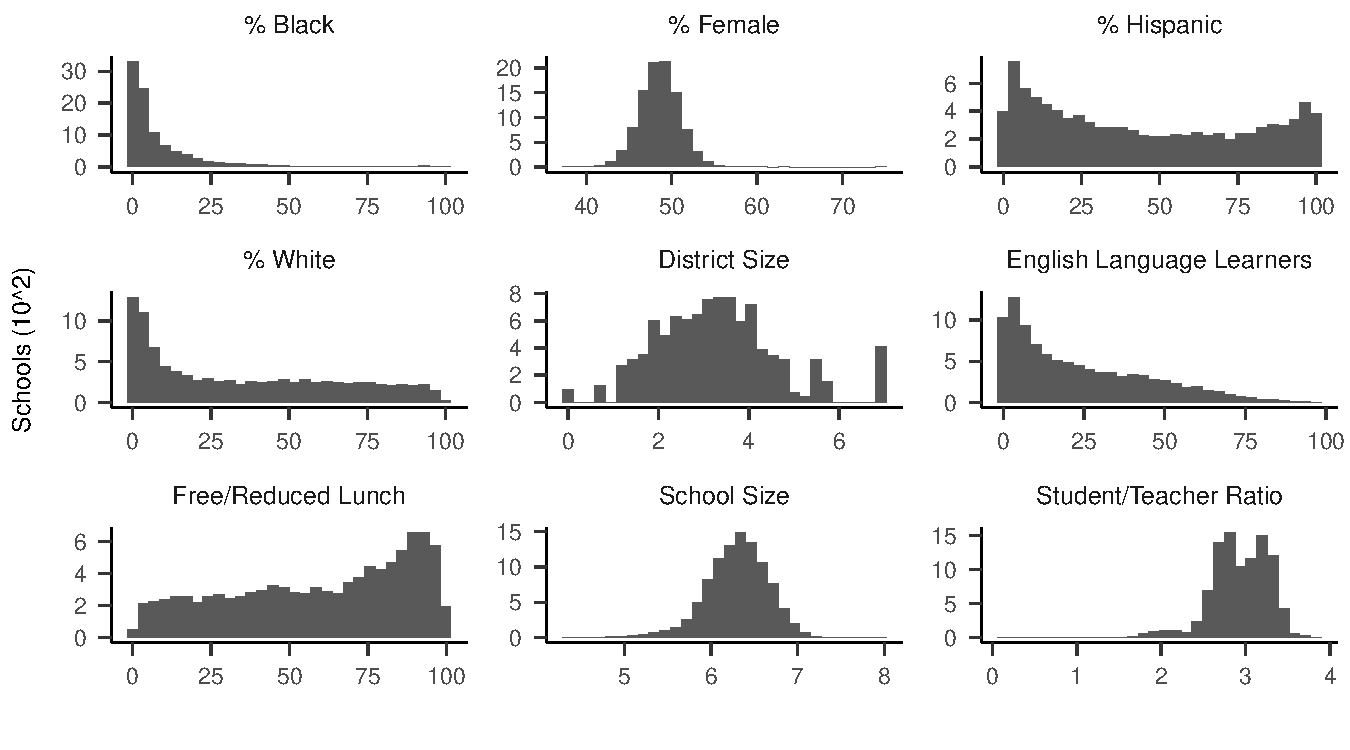
\includegraphics{6---Paper_files/figure-latex/fig-dist1-1.pdf}
\caption{\label{fig:fig-dist1}Distributions of continuous covariates. District Size, School Size, and Student/Teacher Ratio were transformed by taking natural logs.}
\end{figure}

\hypertarget{stratification}{%
\subsection*{Stratification}\label{stratification}}
\addcontentsline{toc}{subsection}{Stratification}

For recruitment methods involving stratification, we use strata generated through a cluster analysis of the school and student characteristics listed in Table \ref{tab:tab-RGM-Pars}.
Our cluster analysis generally followed the approach and recommendations described by Tipton (2014b), with a few modifications. Specifically, we implemented k-medoids clustering to divide the population into heterogeneous strata comprised of homogeneous sites. We used Gower's general similarity measure, which is appropriate for covariates that include both continuous and categorical variables (Gower, 1971; Tipton, 2014b).
All analyses were performed in R (Team, 2017) using the \emph{cluster} package (Mächler, Rousseeuw, Struyf, Hubert, \& Hornik, 2012).
Section \ref{stratification-cluster} of the online appendix includes further details about the cluster analysis and stratification process.

Based on empirical criteria as well as subjective appraisals of what is feasible to implement, we chose a cluster solution with five strata.
The strata ranged in size from 1,222 to 2,863 schools and explained 70\% of the variation across all covariates. The proportion of variance explained by the strata differed by covariate, with five covariates having between 0 and 11\% variance explained by the strata and eight covariates having from 45\% to 87\% variance explained. This discrepancy suggests that stratification will not be equally useful for balancing all covariates.\todo[color=blue!20]{Could you add the percentage of variance explained for each covariate as an additional column in Table 1?}

\hypertarget{participation-propensity-score}{%
\subsection*{Participation Propensity Score}\label{participation-propensity-score}}
\addcontentsline{toc}{subsection}{Participation Propensity Score}

In order to simulate the full process of recruiting a sample for a multi-site trial, we need to choose parameter values for the participation propensity score model (Equation \eqref{eq:RGM}).
To do so, we drew on work by Fellers (2017), who compared 571 elementary schools that participated in IES-funded studies to the full population of U.S. elementary schools on the same variables used in our sampling frame.
Note that this comparison is between schools that participated in trials (i.e., \(P_j = 1\)) and the full population of schools, and so differences may be the result of \emph{both} non-response bias and researcher recruitment bias.
In contrast, we are ideally interested in \(\Pr(E_j = 1 | \mathbf{x}_j)\), the \emph{potential} participation probabilities across the full population.
However, there is little data currently available to directly inform this participation model, and so we relied on the findings of Fellers (2017) to make tentative assumptions about the magnitude of the participation propensity model coefficients.

Fellers (2017) reported absolute standardized mean differences between schools that participated in IES-funded randomized trials and the population. We standardized the covariates and used reported SMDs as coefficients in Equation \eqref{eq:RGM} to generated \(\pi_j\) values. The coefficients are reported in Table \ref{tab:tab-RGM-Pars}.
These values lead to large variation in the response propensity scores. In order to examine the extent to which our results are driven by this assumption, we considered two further conditions, in which the propensity model coefficients were multiplied by a selection factor of 0.5 or 0.25.
These conditions lead to successively weaker relationships between the covariates and the response propensity, so that any imbalances will be driven less by self-selection than by recruitment bias.

The results of Fellers (2017) do not provide any information about the overall potential participation rate across the full population---that is, the fraction of the full population of schools that would agree to participate in a study, if the entire population were recruited. This is a key parameter of the simulation that has a strong influence on the performance of all recruitment methods. We therefore varied the overall participation propensity over a wide range, by manipulating the intercept term in Equation \eqref{eq:RGM}, given the other coefficients of the propensity score model and the selection factor. We considered nine different levels for the average participation rate, ranging from 10\% to 90\%. We also included a participation rate of 99\% to compare sampling performance when there is essentially zero selection bias, and any imbalances are the result of recruitment bias alone.

\hypertarget{simulation-procedures}{%
\subsection*{Simulation procedures}\label{simulation-procedures}}
\addcontentsline{toc}{subsection}{Simulation procedures}

We designed the simulation to examine the performance of 5 recruitment methods across 9 levels of population response rate and 3 levels of the selection factor in the response propensity model. The population of schools and their assigned strata were constant across all conditions and replications. The participation propensity score was constant across all sampling methods and replications within each condition for the response propensity model. Each replication involved first simulating potential participation indicators (\(E_j\)'s) according to Equation \eqref{eq:Ej}, which we then treated as constant across recruitment methods. That is, if a given school was recruited under two different methods, the school would provide the same response under both methods, either agreeing or refusing to participate. Next, we generated five sets of rankings (one for each recruitment method) for all sites.
We checked each site in order of rank for recruitment until a sample of 60 sites was selected by each method. For each sample within an iteration, we tracked which schools were contacted, which schools agreed to participate, and how many schools refused to participate.
The order in which schools were approached varied by recruitment method and across replications. The one exception was the stratified balanced sampling method, where the order in which schools were approached was constant because the ranks were fully determined by stratum assignment and school characteristics.

\hypertarget{performance-measures}{%
\subsection*{Performance measures}\label{performance-measures}}
\addcontentsline{toc}{subsection}{Performance measures}

\hypertarget{generalizability}{%
\subsubsection*{Generalizability}\label{generalizability}}
\addcontentsline{toc}{subsubsection}{Generalizability}

There are several methods to quantify how generalizable a sample is to a target population. One common method is to compare the sample to the population on a range of covariates by examining SMDs as defined in Equation \eqref{eq:SMD}. This method is limited as it only provides us with a measure of how close the sample means are to the population means.
To have full generalizability, however, we should consider how the full distribution of the sample compares to that of the population.

A more comprehensive measure of generalizability is the \(B\) index (Tipton, 2014a), which provides a single score summary of overlap between two groups. This index offers several advantages. First, it takes into account both the variance and distribution of the variables in each group by measuring the overlap of multiple density plots. Second, it quantifies what is typically a visual comparison and provides an intuitive interpretation. Third, it simultaneously compares two groups across a range of covariates and can easily be scaled to include various interactions and transformations.

The \(B\) index is defined in terms of a distribution of propensity scores, which are used to summarize into a single dimension the differences between an obtained sample and the population distribution of the covariates.
For a given recruitment method, let \(\psi_j\) represent the sample selection propensity score, or the logistic transform of the probability that school \(j\) was included in an obtained sample:
\[
\psi_j = \log\left(\frac{\Pr(P_j = 1 | \mathbf{x}_j)}{1 - \Pr(P_j = 1 | \mathbf{x}_j)}\right). 
\]
Note that this sample selection propensity score is distinct from the potential participation propensity model (Equation \eqref{eq:RGM}), in that \(\psi_j\) is based on a sample actually obtained under a given recruitment method, allowing for units to self-select or decline to participate. For each recruitment method and each obtained sample, we estimated \(\psi_j\) using a basic logistic regression:
\begin{align}
\label{eq:PSA}
\psi_j = \gamma_0 + \mathbf{x}_j \boldsymbol\gamma
\end{align}
The estimated values of the sample selection propensity score, \(\hat\psi_j\), serve as scalar summaries of differences across all covariates in \(\mathbf{x}_j\).
The generalizability index compares the distribution of \(\hat\psi_j\) in the sample to the corresponding distribution in the population.
The index is bounded between 0 and 1, with 0 indicating no overlap between the sample and the population, and 1 indicating the sample is representative of the population.
Section \ref{B-index} of the online appendix provides further details about how we calculated the \(B\) index.

\hypertarget{feasibility}{%
\subsubsection*{Feasibility}\label{feasibility}}
\addcontentsline{toc}{subsubsection}{Feasibility}

Recruiters expend a lot of resources contacting districts and schools, scheduling meetings and traveling between prospective schools. A project with limited resources may not be able to afford to go through a large list of potentially uninterested schools. To capture the feasibility of different recruitment methods, we tracked the total number of schools approached for each full sample obtained (Equations \eqref{eq:Zj} and \eqref{eq:Zj-strat}). We then calculated the average number of refusals needed to achieve a full sample for each recruitment method. This measure allows us to compare the feasibility or difficulty of recruiting a full sample using each method.

\hypertarget{sampling-inequity}{%
\subsubsection*{Sampling Inequity}\label{sampling-inequity}}
\addcontentsline{toc}{subsubsection}{Sampling Inequity}

This simulation design also enables us to study sampling inequality. The distribution of opportunities to participate in research is an important issue when considering federally funded research.
Non-random sampling for such studies create the possibility of systemic under-representation of some types of schools, which then do not share in the benefits of participating in research, or systemic over-representation of other schools, which more often bear the burden of participation in such research.

To assess sampling inequity, we tracked the proportion of replication in which each school in the population participated in the study. We then summarized these data by calculating a Gini coefficient for each recruitment method and each population participation rate. This index ranges from 0 to 1, with 0 indicating perfect equity, and 1 indicating total inequity.
In economic contexts, the Gini coefficient is often used to describe the degree of income or wealth inequality in a population. In the context of evaluating sampling methods, we use the Gini coefficient to summarize the distribution of opportunities to participate in research. We calculated Gini coefficients using the \emph{Gini} function from the \emph{ineq} package (Zeileis, 2014).

\hypertarget{results}{%
\section*{Results}\label{results}}
\addcontentsline{toc}{section}{Results}

\hypertarget{generalizability-1}{%
\subsection*{Generalizability}\label{generalizability-1}}
\addcontentsline{toc}{subsection}{Generalizability}

\hypertarget{b-index}{%
\subsubsection*{B-Index}\label{b-index}}
\addcontentsline{toc}{subsubsection}{B-Index}

Figure \ref{fig:fig-avg-B} displays the average \(B\)-index resulting from each recruitment method, for varying participation rates (on the horizontal axis) and selection factors.\todo[color=blue!20]{Use bubble labels in the plots and remove the figure legend.} Acceptable values of \(B\) for generalizability vary depending on the size of the sample, the size of the population, and the number of covariates (Tipton, 2014a). Given our design, a value of \(B = .95\) would indicate very good overlap with no need to adjust estimates. Generally \(B >= .80\) still supports generalizability with adjustment and likely no need to redefine the population.



\begin{figure}
\centering
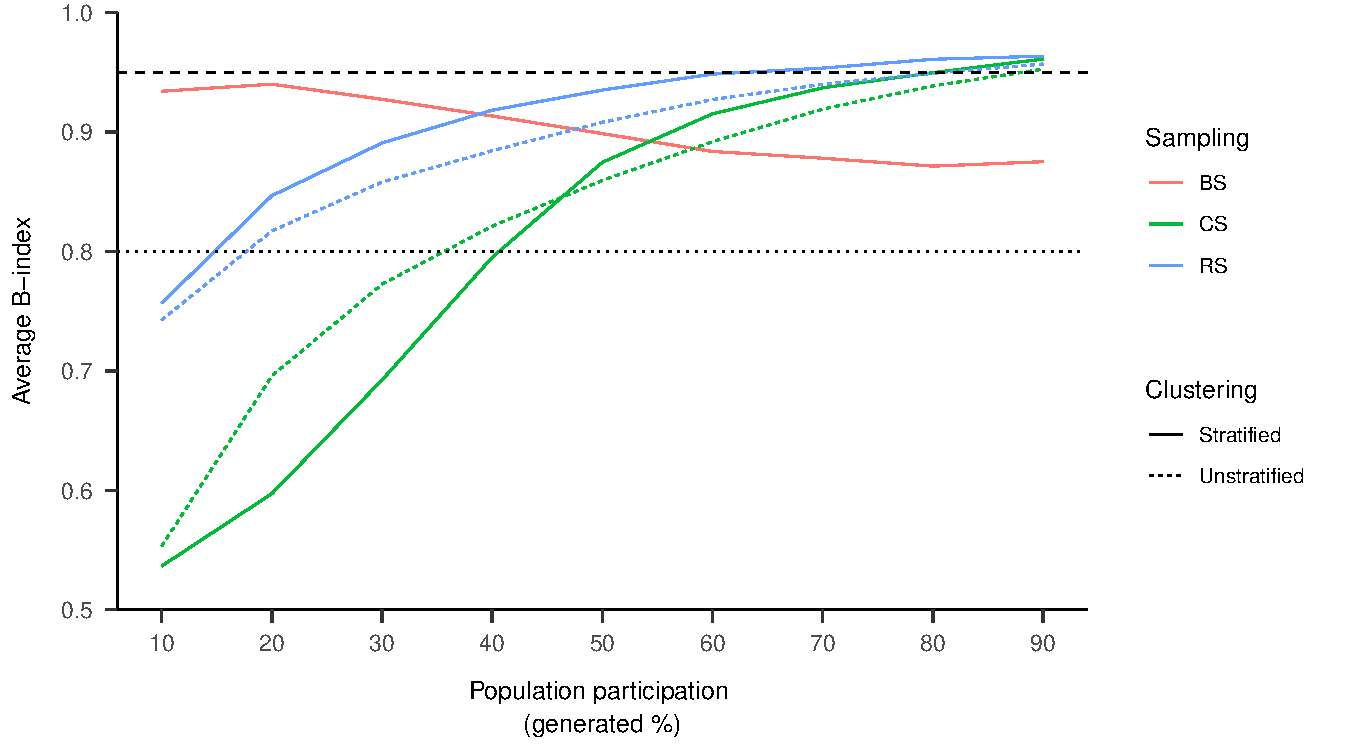
\includegraphics{6---Paper_files/figure-latex/fig-avg-B-1.pdf}
\caption{\label{fig:fig-avg-B}Average \(B\)-index for varying participation rates across SFs, by sampling method. Horizontal dotted lines represented indices of .80 and .95, indicating acceptable or high levels of generalizability.}
\end{figure}

For all methods, average \(B\) values varied by participation rate and selection factor. At the highest participation rates, generalizability is affected only by recruitment bias. Consequently, each recruitment method converges to a constant average \(B\) index across all three selection factors. For all methods, the size of the selection factor affects the strength of the relationship between the participation rate and the degree of generalizability: with larger selection factors, lower participation rates lead to larger losses in generalizability.

SBS consistently outperformed other recruitment methods across response rates and selection factors. Further, with the exception of a 10\% and 20\% population response rate at \(SF = 1\), SBS never resulted in a \(B\) value below .95. This indicates that SBS is successful at sampling sites that are unlikely to participate and therefore tend to be underrepresented by the other sampling methods---particularly when overall participation propensities are low.

The stratified and unstratified random sampling methods also led to \(B\) values indicating high degrees of generalizability. Except under conditions with the strongest selection factor and the lowest potential participation rates, \(B\) values were above .80. At higher participation rates or when the selection factor was 0.5 or 0.25, stratified random sampling led to average \(B\) values that were very close to those from SBS. Stratified random sampling consistently outperformed simple random sampling across all participation rates, though only slightly.

We\todo[color=blue!20]{This paragraph needs to start with an overall characterization of how convenience sampling methods performed.} also found that, unexpectedly, at low response rates, unstratified convenience sampling achieved better balance than stratified convenience sampling when \(SF = 1\). This seems counter-intuitive, as survey literature suggests that stratification produces more representative samples (Lohr, 2019). Because the \(B\)-index is an overall measure of generalizability across many covariates, it does not provide much indication of why these performance differences occur. To untangle why the methods performed as they did, we examined the balance obtained by each recruitment method on individual covariates.

\hypertarget{standardized-mean-differences}{%
\subsubsection*{Standardized Mean Differences}\label{standardized-mean-differences}}
\addcontentsline{toc}{subsubsection}{Standardized Mean Differences}

Standardized mean differences for each recruitment method for each specific covariate indicate how recruitment methods compare in terms of balancing specific site characteristics, which may be associated with treatment effect heterogeneity and potential participation decisions.
We interpreted a method as performing adequately if it resulted in an average imbalance of no more than 0.25 standard deviations. When making comparisons, we classified methods as performing differently only if one or both did not achieve adequate balance (\(SMD > .25\)), otherwise the methods were considered comparable.



\begin{figure}
\centering
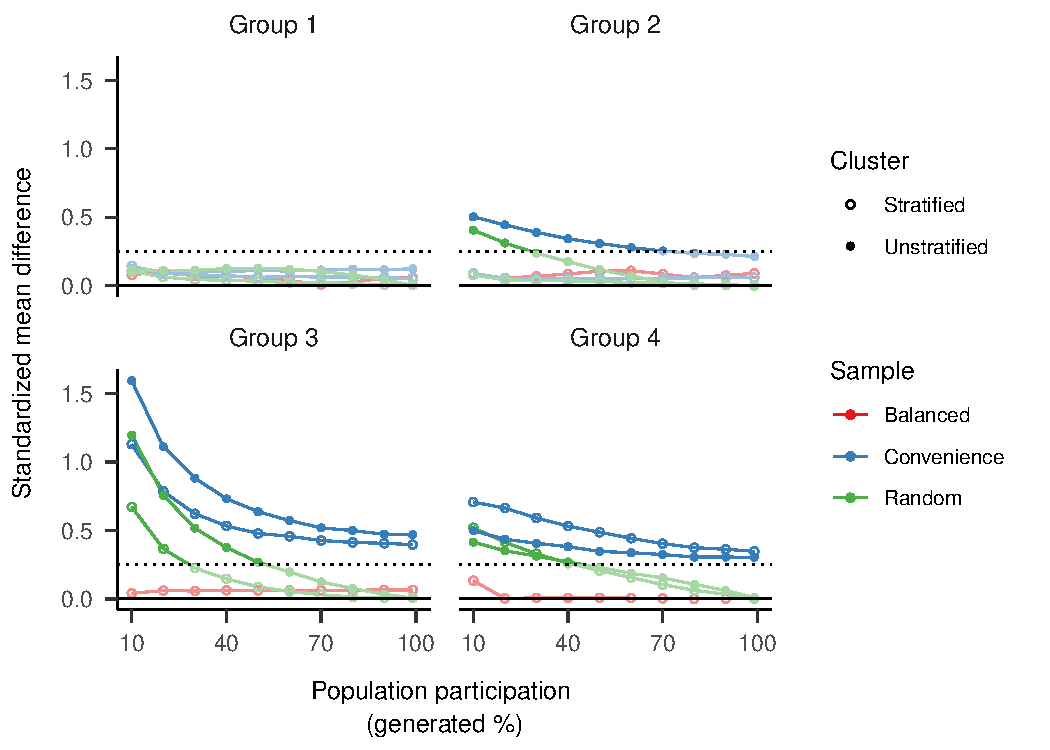
\includegraphics{6---Paper_files/figure-latex/fig-SMD-groups-1.pdf}
\caption{\label{fig:fig-SMD-groups}Patterns of relative performance based on standardized mean differences. The dotted horizontal line represents a threshold of 0.25 for acceptable balance. Results are displayed for the highest selection factor \((SF = 1)\) to highlight differences between the groups of covariates.}
\end{figure}

The relative performance of sampling methods varied depending on the covariate and selection factors. We found that there were several different patterns of relative performance in balancing different covariates. Four distinct groups of covariates emerged:

\begin{enumerate}
\def\labelenumi{(\arabic{enumi})}
\tightlist
\item
  covariates where all methods consistently achieved good balance;
\item
  covariates where stratified sampling methods consistently achieved good balance, but where unstratified methods sometimes resulted in poor balance;
\item
  covariates where good balance was consistently achieved for SBS only, and where other stratified methods outperformed the unstratified counterparts; and\\
\item
  covariates exhibiting unique patterns that did not match groups 1, 2 and 3.
\end{enumerate}

Figure \ref{fig:fig-SMD-groups} displays an example of each pattern for \(SF = 1\);\todo[color=blue!20]{Use bubble labels in the plots and remove the figure legend. Also, could you add the specific covariate in the label for each group? e.g., "Group 1: Student/Teacher Ratio"} results for each specific covariate can be found in Online Appendix Figures \ref{fig:fig-smd-group1}, \ref{fig:fig-smd-group2}, \ref{fig:fig-smd-group3}, and \ref{fig:fig-smd-group4}.



\begin{figure}
\centering
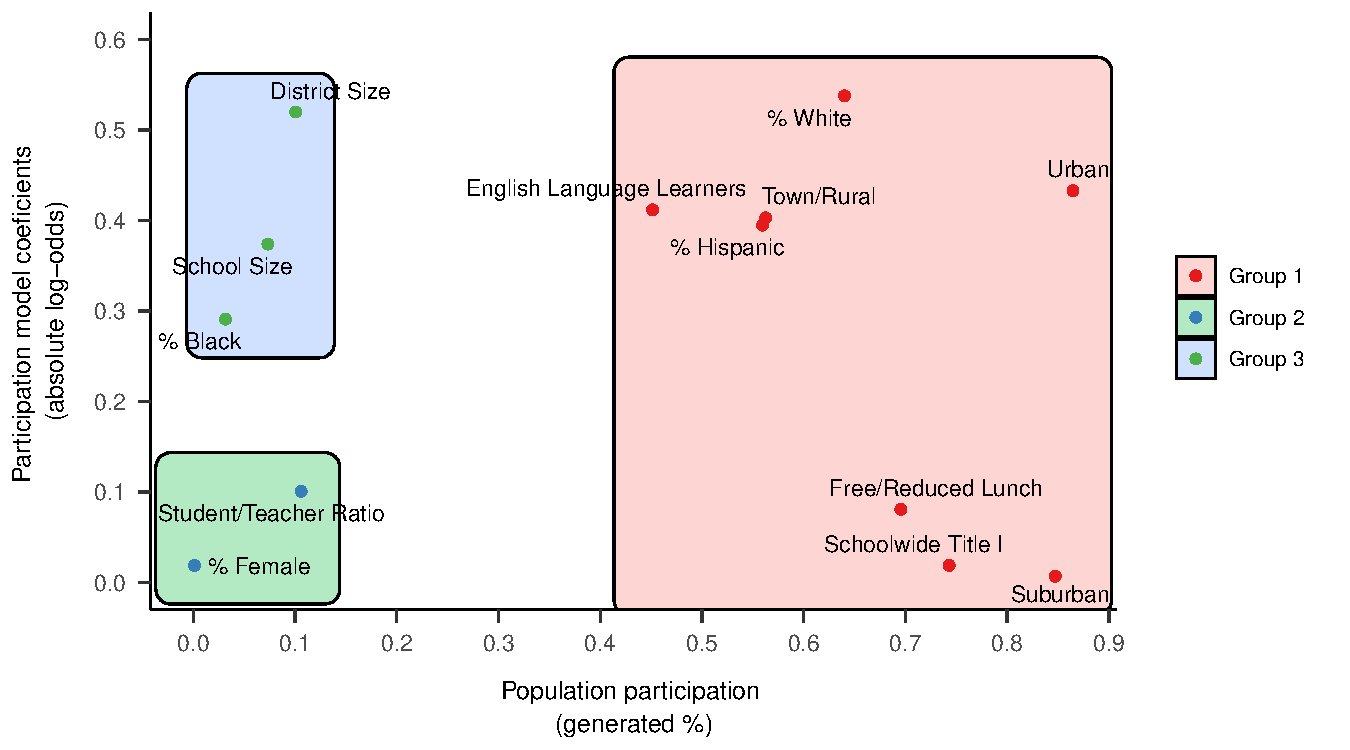
\includegraphics{6---Paper_files/figure-latex/fig-Var-Coef-1.pdf}
\caption{\label{fig:fig-Var-Coef}Variance explained by clustering vs absolute log-odds. Shaded areas illustrate groupings of covariates with respect to patterns of imbalance as measured by standardized mean differences.}
\end{figure}

One potential explanation for these patterns is the relationship between a covariate's coefficient in the response generation model and its level of heterogeneity across strata.
Figure \ref{fig:fig-Var-Coef} plots the log-odds coefficient for each covariate against the proportion of its variance explained by the strata.
Differences between groups are highly contrasted at \(SF = 1\). Group 1 consists of low level predictors of participation which are relatively homogeneous across strata. Given that these covariates contribute little to selection bias and were unaffected by the stratification process, it is reasonable to expect that most recruitment methods will achieve good balance.
Group 2 consists of covariates where a high proportion of variance is explained by stratum membership. Group 3 consists of covariates with intermediate levels of between-stratum variance that were strongly associated with potential participation decisions. Stratified methods consistently performed well for covariates with high variance ratios, though SCS and SRS struggled a bit more with covariates strongly associated with self-selection.
Group 4 is unique in that it consists of two unique patterns: (1) where SCS and SRS under-performed UCS and URS, respectively, and (2) where SBS did not result in good balance at lower response rates. It is also notable that the patterns described above become less consistent when the selection factor was lower, so that imbalances were relatively more driven by recruitment bias rather than by self-selection. Other factors that may contribute to these patterns include the covariance among the predictors or the generated response rates.

\hypertarget{feasibility-1}{%
\subsection*{Feasibility}\label{feasibility-1}}
\addcontentsline{toc}{subsection}{Feasibility}

Figure \ref{fig:fig-responses}a depicts the total number of sites contacted to recruit a full sample of 60 sites versus the population participation rate, for each recruitment method. Figure \ref{fig:fig-responses}b depicts the response rate, or percentage of sites that agreed to participate among those where recruitment was attempted, versus the population participation rate, for each recruitment method.\todo[color=blue!20]{Need to clarify that these are for SF = 1.} For each of these metrics, there were substantial differences between methods at lower population participation rates. At higher participation rates, the differences were less pronounced, becoming negligible at population participation rates of 60\% or more.



\begin{figure}[tb]
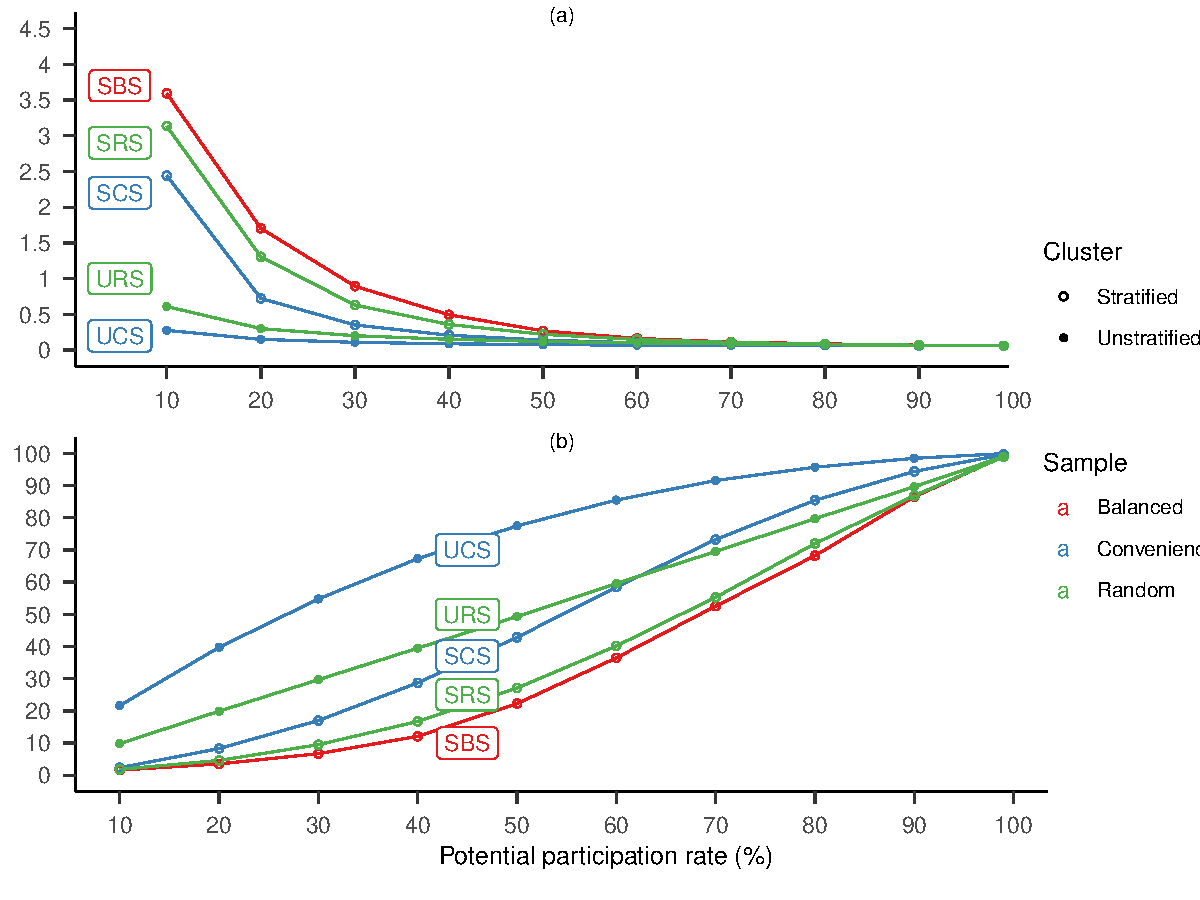
\includegraphics[width=0.6\linewidth]{6---Paper_files/figure-latex/fig-responses-1} \caption{Sample recruitment statistics and response rates. (a) Total number of sites contacted to achieve a full sample of 60 sites. (b) Percentage of contacted sites that agreed to participate.}\label{fig:fig-responses}
\end{figure}

Under our model, the total sites contacted under all of the methods are quite large---extremely so, when population participation rates are low. Due to the speculative nature of the simulation, we restrict our interpretation to comparisons of the \emph{relative} performance of the recruitment methods. Under our modeling assumptions, SBS required a larger number of recruitment attempts (with a lower average participation rate) compared to the other recruitment methods. Stratified random sampling and stratified convenience sampling both required more recruitment effort than the unstratified methods, probably due to differences between the strata in potential response rates.
As would be expected, unstratified convenience sampling required the smallest recruitment effort to obtain a full sample. Online Appendix Figure \ref{fig:fig-rel-per} provides further detail about the relative feasibility of each recruitment method.\todo[color=blue!20]{Modify this figure to show the other selection factors too.}

\hypertarget{sampling-inequity-1}{%
\subsection*{Sampling Inequity}\label{sampling-inequity-1}}
\addcontentsline{toc}{subsection}{Sampling Inequity}

We calculated the Gini coefficient for each sampling method to examine the equity implications of different recruitment methods. Figure \ref{fig:fig-gini} displays these for each sampling method across population participation rates.\todo[color=blue!20]{Use bubble labels in the plots and remove the figure legend.} A coefficient of 1 indicates absolute sampling inequity, meaning that the same, small subset of the population participated in the study across all replications.
Individual Gini curves and coefficients for each method across response rates can be found in Online Appendix Figure \ref{fig:fig-gini-curve}.



\begin{figure}
\centering
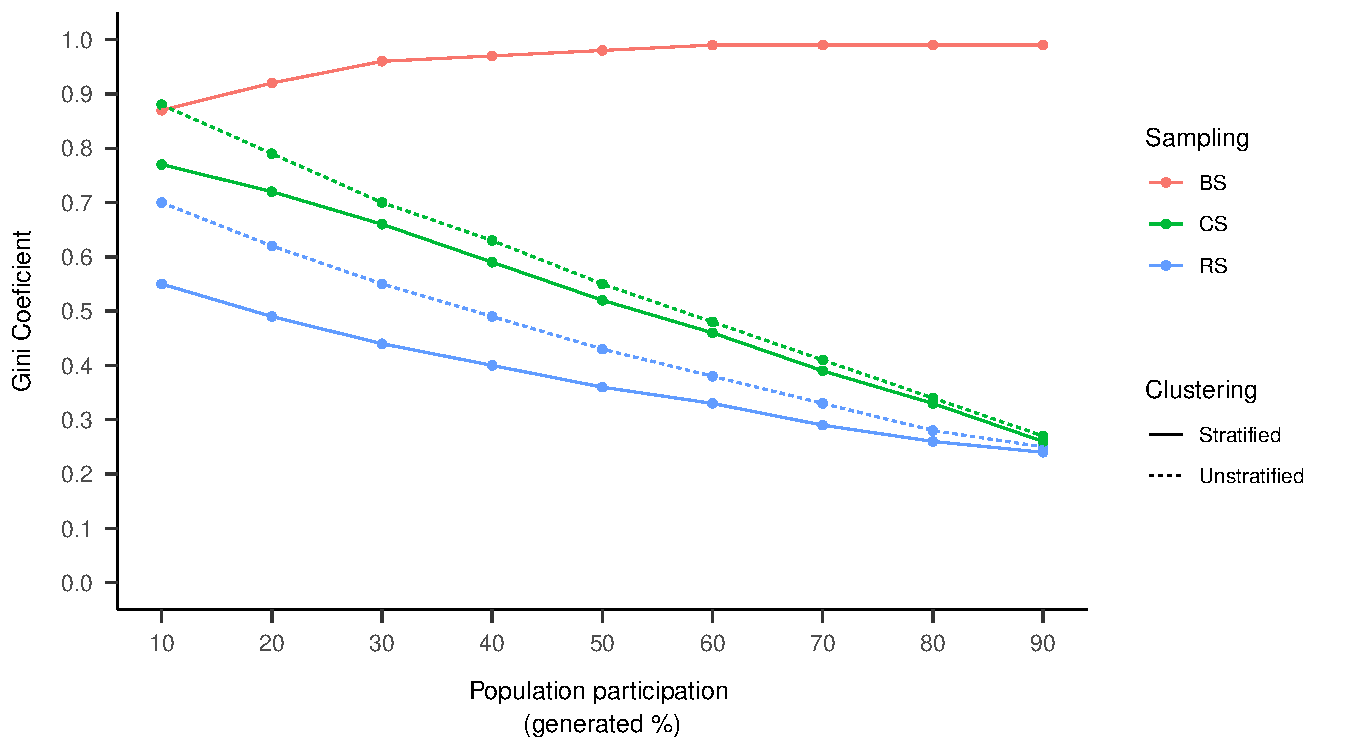
\includegraphics{6---Paper_files/figure-latex/fig-gini-1.pdf}
\caption{\label{fig:fig-gini}Gini coefficient across participation response rates for each sampling method. A coefficient of 1 indicates major inequality in sampling probability.}
\end{figure}

Several trends emerged in this analysis. Overall, SBS was the most inequitable sampling process. This is consistent with the balanced sample approach because order of recruitment is tied to site characteristics and constant across replications. Stratified random sampling was the most equitable sampling process, followed by unstratified random sampling, stratified convenience sampling, and unstratified convenience sampling.
At higher population participation rates, inequity increased when using SBS, but decreased considerably when using the other methods. Differences between stratified and unstratified random sampling diminished at higher participation rates, and a similar pattern held for stratified and unstratified convenience sampling. This suggests that stratifying the population results in a more diverse sampling pool when the overall population response rate is low.
However, stratification alone is still limited by the recruitment method within strata, and methods that do not involve probability sampling lead to increased sampling inequality.

\hypertarget{discussion}{%
\section*{Discussion}\label{discussion}}
\addcontentsline{toc}{section}{Discussion}

The main goal of this study was to develop a framework for exploring the performance of different recruitment methods within the context of multi-site randomized trials of educational interventions. We have described algorithmic representations of several different processes that researchers might use to recruit sites into a trial. Informed by prior empirical work, we also attempted to model how sites decide whether or not to participate in a study if approached by recruiters. The methods we proposed for modeling these behaviors can, in principle, be extended to more complex and realistic specifications and adapted to other population frames.

A second goal was to use this framework to investigate the relative performance of different several sampling methods in terms of generalizability, feasibility, and equity. Based on these simulation, we draw several tentative conclusions. Stratified balanced sampling as proposed by Tipton (2014b) has the potential to greatly increase the generalizability of samples selected for multi-site randomized trials. In particular, SBS resulted in a considerable improvement compared to unstratified convenience sampling---the method that we suspect most closely approximates current recruitment practices in education research. However, SBS is not without limitations. Within our simulation, strict application of SBS came at a great cost in terms of the number of sites that needed to be contacted. If population participation rates are low, it may be infeasible to fully implement SBS in the ideal form. Even with higher participation rates, implementing this method in practice may require allocating many more study resources to sample Furthermore, although the balanced sampling approach does result in strong generalizability, it might also limit the pool of potential participants. Particularly for larger population response rates, only a small subset of sites were likely to participate across replications of the simulation.

Another consistent pattern was that convenience and probability sampling methods were often improved through stratifying the population and setting target sample sizes for each stratum. In fact, in cases where the cluster analysis performed well for a given covariate, or where population participation rates were high, convenience sampling within strata performed as well as or better than unstratified random sampling on measures of both generalizability and feasibility.

We also found that the properties of the strata generated by cluster analysis have implications for the generalizability of samples recruited through stratified methods. If a covariate was predictive of participation propensity, then it was important for the stratification to explain a substantial fraction of its total variation. If a covariate was predictive of participation, but not prioritized when generating the strata, it had poor representation in samples collected through stratified methods. Ignoring the quality of the cluster analysis solution has the potential to undermine the performance of SBS. It is therefore important to not only examine overall variance explained when performing the cluster analysis, but to use individual covariate variability as a criterion as well.

One potential compromise between current practice (such as unstratified convenience sampling) and SBS is to combine stratification with some form of convenience sampling. As demonstrated in the simulations, stratified convenience sampling often resulted in better balance on individual covariates than simple random sampling, and required lower recruitment effort compared to balanced sampling. This may also elicit greater buy-in from recruiters by placing less restrictions on which units they must sample.
Beyond generalizability, stratifying in this manner requires researchers to make sampling decisions in the study design phase and to track changes in the sampling plan as recruitment progresses. Documenting and reporting this process would in turn support further research into developing more efficient and effective sampling methods.

\hypertarget{limitations}{%
\subsection*{Limitations}\label{limitations}}
\addcontentsline{toc}{subsection}{Limitations}

The models that we have studied make several key assumptions which represent limitations on the findings from the simulation study. First, in modeling convenience sampling, we assumed that recruiters prioritize sites that are most likely to participate. In reality, other factors may play a role as well, such as proximity of sample sites to the researcher and to each other, existing relationships between the recruiters and the sample sites, and the researchers' own personal biases.
Due to this limitation, caution is warranted in interpreting the simulation findings regarding the absolute performance and absolute feasibility of convenience sampling methods.
This assumption also rests on the premise that recruiters have some knowledge of how likely a sampled site is to participate. Though researchers may speculate about sites that are more willing to participate (such as schools in larger urban districts) and prioritize recruiting such sites, their estimation of ``willingness'' may be further from the truth than what we have assumed. If so, it is possible that the feasibility of the convenience methods is over-stated and that their degree of generalizability is under-stated in these simulations.

It would be worth refining and exploring additional methods for modeling convenience sampling. The algorithms used in these methods could be tuned to include additional factors that might influence site recruitment priorities. For instance, location data is readily available and could be incorporated into the model for how researchers prioritize schools in convenience sampling. Further work here could lead to more realistic and practical assessments of feasibility and generalizability, potentially providing researchers with a tool for evaluation of recruitment methods given the unique circumstances that they face during the study design phase.

A second limitation arises from the simplified and speculative nature of our participation model. In practice, the decision of whether a school participates in such a study often involves multiple stages. District offices often serve as gatekeepers, requiring submission and approval of research requests prior to contacting individual schools. If the request is denied, no schools within the district may be recruited. If approved, researchers may work with a district-wide school coordinator, or may have to contact schools individually. In either cases, the ultimate decision may then rest with administrators, school research coordinators, or the teachers themselves. Our participation model assumed that only school level characteristics play a roll in this decision, when in reality a multilevel model accounting for district and individual administrative characteristics would be a more realistic representation of the process. However, we are not aware of data sources that would allow us to develop even very rough estimates of such a model's parameters.

A further limitation of the simulations is that the parameters in the response generating model are based on values from a study that examined the difference between schools participating in large-scale randomized trials and the overall population of schools. However, these trials themselves typically rely on some form of convenience sampling. As a result, our parameters reflect participation rates of schools that are likely to participate in randomized trials, rather than the full population of schools.

This limitation points towards the need for more extensive research regarding factors that influence school participation in randomized trials. In particular, research is needed that can disentangle recruitment bias from selection bias. Such information could be generated through careful record-keeping during the recruitment stages of multi-site trials that aim for large-scale population representation.
Such efforts could provide deeper insight into school behavior and representation in research. If we can identify schools that are consistently and systematically under-represented in funded research, we can develop strategies to target such schools and increase the inclusivity of studies that strive for truly representative population-level inferences.

\hypertarget{future-directions}{%
\subsection*{Future Directions}\label{future-directions}}
\addcontentsline{toc}{subsection}{Future Directions}

In this study, we have sought to lay the groundwork for several avenues of further research. First, additional work is needed on how best to implement cluster analysis in the context of stratified sampling methods. We have shown that the extent to which balance is achieved on a given covariate is related to how strongly the strata explain variation in the covariate and how strongly the covariate is related to school participation. If some covariates are known to have greater influence on school participation, it may be useful to weight them more heavily in generating the strata. Further work is also needed to understand the relationship between the number of strata, generalizability, and feasibility. It is expected that more clusters would increase generalizability, but also make recruitment more difficult. A better understanding of these relationships would help drive decision-making during the design phase, potentially making SBS more accessible and quicker to implement.

Further work also needs to examine the impact of these sampling methods on the bias and accuracy of population average treatment effect estimates. In this study, our goal was only to select a generalizable sample, where generalizability was operationalized as balance between the sample and population on a set of covariates. To the extent that the same covariates that dictate selection are also predictive of variation in treatment effects, we may extrapolate that a sample that is balanced on these covariates can be used to estimate population average treatment effects with little or no bias. Still, we think it would be worth investigating the full process--from study design to parameter estimation--to understand how sampling methods influence the bias and overall accuracy of impact estimators for target population.

If treatment effects are constant across units in a population, non-representative samples of the population should still lead to unbiased estimates of average treatment effects. However, if only a narrow slice of the population is studied, there may not be sufficient variability in potential moderators to detect heterogeneity. Adding variation by selecting a more diverse sample may be useful if the extent of heterogeneity is unknown. This further complicates the specification of the cluster analysis. How should covariates be weighed relative to each other depending on whether they predict participation, differences in treatment effects, or some combination of both? To address this our work must be extended to study the relationship between sampling methods and bias in treatment effect estimation.\todo[color=blue!20]{I don't quite follow how this fits in. Let's discuss this point.}\todo[color=orange]{We didn't discuss this, should I drop for now?}

Large scale multi-site randomized trials are expensive to implement, and resource allocation for such studies presents many difficult trade-offs. Researchers who wish to invest in robust recruitment strategies to amplify the impact and relevance of of their work should be better equipped to anticipate the costs and benefits of various sampling strategies. Through further refinement of the models and simulations demonstrated here, we hope to help researchers make more informed decisions about sample recruitment and representation.

\newpage

\hypertarget{references}{%
\section*{References}\label{references}}
\addcontentsline{toc}{section}{References}

\begingroup
\setlength{\parindent}{-0.5in}

\hypertarget{refs}{}
\begin{CSLReferences}{1}{0}
\leavevmode\vadjust pre{\hypertarget{ref-calinskiDendriteMethodCluster1974}{}}%
Caliński, T., \& Harabasz, J. (1974). A dendrite method for cluster analysis. \emph{Communications in Statistics}, \emph{3}(1), 1--27. \url{https://doi.org/10.1080/03610927408827101}

\leavevmode\vadjust pre{\hypertarget{ref-chan_partially_2017}{}}%
Chan, W. (2017). Partially {Identified} {Treatment} {Effects} for {Generalizability}. \emph{Journal of Research on Educational Effectiveness}, \emph{10}(3), 646--669. \url{https://doi.org/10.1080/19345747.2016.1273412}

\leavevmode\vadjust pre{\hypertarget{ref-fellersDevelopingApproachDetermine2017}{}}%
Fellers, L. (2017). \emph{Developing an approach to determine generalizability: {A} review of efficacy and effectiveness trials funded by the {Institute} of {Education Sciences}} (Ph.D., Columbia University). Columbia University, United States -- New York. Retrieved from \url{https://search.proquest.com/docview/1865595768/abstract/40FD82F4A0C24535PQ/1}

\leavevmode\vadjust pre{\hypertarget{ref-gerberFieldExperimentsDesign2012}{}}%
Gerber, A. S., \& Green, D. P. (2012). \emph{Field experiments: Design, analysis, and interpretation} (1st ed). New York: W. W. Norton.

\leavevmode\vadjust pre{\hypertarget{ref-gowerGeneralCoefficientSimilarity1971}{}}%
Gower, J. C. (1971). A {General Coefficient} of {Similarity} and {Some} of {Its Properties}. \emph{Biometrics}, \emph{27}(4), 857--871. \url{https://doi.org/10.2307/2528823}

\leavevmode\vadjust pre{\hypertarget{ref-grovesSurveyMethodology2004}{}}%
Groves, R. M. (Ed.). (2004). \emph{Survey methodology}. Hoboken, N.J: Wiley-Interscience.

\leavevmode\vadjust pre{\hypertarget{ref-R-fpc}{}}%
Hennig, C. (2019). \emph{Fpc: Flexible procedures for clustering}. Retrieved from \url{https://CRAN.R-project.org/package=fpc}

\leavevmode\vadjust pre{\hypertarget{ref-hennigHowFindAppropriate2013}{}}%
Hennig, C., \& Liao, T. F. (2013). How to find an appropriate clustering for mixed-type variables with application to socio-economic stratification: {How} to {Find} an {Appropriate Clustering}. \emph{Journal of the Royal Statistical Society: Series C (Applied Statistics)}, \emph{62}(3), 309--369. \url{https://doi.org/10.1111/j.1467-9876.2012.01066.x}

\leavevmode\vadjust pre{\hypertarget{ref-imaiMisunderstandingsExperimentalistsObservationalists2008}{}}%
Imai, K., King, G., \& Stuart, E. A. (2008). Misunderstandings between experimentalists and observationalists about causal inference. \emph{Journal of the Royal Statistical Society: Series A (Statistics in Society)}, \emph{171}(2), 481--502. \url{https://doi.org/10.1111/j.1467-985X.2007.00527.x}

\leavevmode\vadjust pre{\hypertarget{ref-kernAssessingMethodsGeneralizing2016}{}}%
Kern, H. L., Stuart, E. A., Hill, J., \& Green, D. P. (2016). Assessing {Methods} for {Generalizing Experimental Impact Estimates} to {Target Populations}. \emph{Journal of Research on Educational Effectiveness}, \emph{9}(1), 103--127. \url{https://doi.org/10.1080/19345747.2015.1060282}

\leavevmode\vadjust pre{\hypertarget{ref-lohrSamplingDesignAnalysis2019}{}}%
Lohr, S. L. (2019). \emph{Sampling: {Design} and {Analysis}} (2nd Edition). Chapman; Hall/CRC.

\leavevmode\vadjust pre{\hypertarget{ref-machlerClusterClusterAnalysis2012}{}}%
Mächler, M., Rousseeuw, P., Struyf, A., Hubert, M., \& Hornik, K. (2012). \emph{Cluster: {Cluster Analysis Basics} and {Extensions}} (Vol. 1).

\leavevmode\vadjust pre{\hypertarget{ref-omuircheartaighGeneralizingUnrepresentativeExperiments2014}{}}%
O'Muircheartaigh, C., \& Hedges, L. V. (2014). Generalizing from unrepresentative experiments: A stratified propensity score approach. \emph{Journal of the Royal Statistical Society: Series C (Applied Statistics)}, \emph{63}(2), 195--210. \url{https://doi.org/10.1111/rssc.12037}

\leavevmode\vadjust pre{\hypertarget{ref-olsenExternalValidityPolicy2013}{}}%
Olsen, R. B., Orr, L. L., Bell, S. H., \& Stuart, E. A. (2013). External {Validity} in {Policy Evaluations That Choose Sites Purposively}. \emph{Journal of Policy Analysis and Management}, \emph{32}(1), 107--121. \url{https://doi.org/10.1002/pam.21660}

\leavevmode\vadjust pre{\hypertarget{ref-raudenbush2015learning}{}}%
Raudenbush, S. W., \& Bloom, H. S. (2015). Learning about and from a distribution of program impacts using multisite trials. \emph{American Journal of Evaluation}, \emph{36}(4), 475--499.

\leavevmode\vadjust pre{\hypertarget{ref-raudenbushStatisticalPowerOptimal2000}{}}%
Raudenbush, S. W., \& Liu, X. (2000). Statistical power and optimal design for multisite randomized trials. \emph{Psychological Methods}, \emph{5}(2), 199--213. \url{https://doi.org/10.1037//1082-989X.5.2.199}

\leavevmode\vadjust pre{\hypertarget{ref-shadishExperimentalQuasiexperimentalDesigns2002}{}}%
Shadish, W. R., Cook, T. D., \& Campbell, D. T. (2002). \emph{Experimental and quasi-experimental designs for generalized causal inference}. Boston, MA, US: Houghton, Mifflin; Company.

\leavevmode\vadjust pre{\hypertarget{ref-steinleyKmeansClusteringHalfcentury2006}{}}%
Steinley, D. (2006). K-means clustering: {A} half-century synthesis. \emph{British Journal of Mathematical and Statistical Psychology}, \emph{59}(1), 1--34. \url{https://doi.org/10.1348/000711005X48266}

\leavevmode\vadjust pre{\hypertarget{ref-stuartCharacteristicsSchoolDistricts2017}{}}%
Stuart, E. A., Bell, S. H., Ebnesajjad, C., Olsen, R. B., \& Orr, L. L. (2017). Characteristics of {School Districts That Participate} in {Rigorous National Educational Evaluations}. \emph{Journal of Research on Educational Effectiveness}, \emph{10}(1), 168--206. \url{https://doi.org/10.1080/19345747.2016.1205160}

\leavevmode\vadjust pre{\hypertarget{ref-stuartUsePropensityScores2011}{}}%
Stuart, E. A., Cole, S. R., Bradshaw, C. P., \& Leaf, P. J. (2011). The use of propensity scores to assess the generalizability of results from randomized trials: {Use} of {Propensity Scores} to {Assess Generalizability}. \emph{Journal of the Royal Statistical Society: Series A (Statistics in Society)}, \emph{174}(2), 369--386. \url{https://doi.org/10.1111/j.1467-985X.2010.00673.x}

\leavevmode\vadjust pre{\hypertarget{ref-rcite}{}}%
Team, R. C. (2017). \emph{R: A language and environment for statistical computing}. Vienna, Austria: R Foundation for Statistical Computing. Retrieved from \url{https://www.R-project.org/}

\leavevmode\vadjust pre{\hypertarget{ref-tiptonImprovingGeneralizationsExperiments2013}{}}%
Tipton, E. (2013). Improving {Generalizations From Experiments Using Propensity Score Subclassification}: {Assumptions}, {Properties}, and {Contexts}. \emph{Journal of Educational and Behavioral Statistics}, \emph{38}(3), 239--266. Retrieved from \url{https://www.jstor.org/stable/41999424}

\leavevmode\vadjust pre{\hypertarget{ref-tiptonHowGeneralizableYour2014}{}}%
Tipton, E. (2014a). How {Generalizable Is Your Experiment}? {An Index} for {Comparing Experimental Samples} and {Populations}. \emph{Journal of Educational and Behavioral Statistics}, \emph{39}(6), 478--501.

\leavevmode\vadjust pre{\hypertarget{ref-tiptonStratifiedSamplingUsing2014}{}}%
Tipton, E. (2014b). Stratified {Sampling Using Cluster Analysis}: {A Sample Selection Strategy} for {Improved Generalizations From Experiments}. \emph{Evaluation Review}, \emph{37}(2), 109--139. \url{https://doi.org/10.1177/0193841X13516324}

\leavevmode\vadjust pre{\hypertarget{ref-tiptonSiteSelectionExperiments2016}{}}%
Tipton, E., Fellers, L., Caverly, S., Vaden-Kiernan, M., Borman, G., Sullivan, K., \& de Castilla, V. R. (2016). Site {Selection} in {Experiments}: {An Assessment} of {Site Recruitment} and {Generalizability} in {Two Scale}-up {Studies}. \emph{Journal of Research on Educational Effectiveness}, \emph{9}, 209--228. \url{https://doi.org/10.1080/19345747.2015.1105895}

\leavevmode\vadjust pre{\hypertarget{ref-tiptonImplicationsSmallSamples2017}{}}%
Tipton, E., Hallberg, K., Hedges, L. V., \& Chan, W. (2017). Implications of {Small Samples} for {Generalization}: {Adjustments} and {Rules} of {Thumb}. \emph{Evaluation Review}, \emph{41}(5), 472--505. \url{https://doi.org/10.1177/0193841X16655665}

\leavevmode\vadjust pre{\hypertarget{ref-tiptonImprovedGeneralizabilityImproved2019}{}}%
Tipton, E., \& Matlen, B. J. (2019). Improved {Generalizability Through Improved Recruitment}: {Lessons Learned From} a {Large}-{Scale Randomized Trial}. \emph{American Journal of Evaluation}, \emph{40}(3), 414--430. \url{https://doi.org/10.1177/1098214018810519}

\leavevmode\vadjust pre{\hypertarget{ref-tipton_review_2018}{}}%
Tipton, E., \& Olsen, R. B. (2018). A {Review} of {Statistical} {Methods} for {Generalizing} {From} {Evaluations} of {Educational} {Interventions}. \emph{Educational Researcher}, \emph{47}(8), 516--524. \url{https://doi.org/10.3102/0013189X18781522}

\leavevmode\vadjust pre{\hypertarget{ref-tiptonSystemEvidenceAll2020}{}}%
Tipton, E., Spybrook, J., Fitzgerald, K. G., Wang, Q., \& Davidson, C. (2020). Toward a {System} of {Evidence} for {All}: {Current Practices} and {Future Opportunities} in 37 {Randomized Trials}. \emph{Educational Researcher}, 0013189X20960686. \url{https://doi.org/10.3102/0013189X20960686}

\leavevmode\vadjust pre{\hypertarget{ref-ineq}{}}%
Zeileis, A. (2014). \emph{Ineq: Measuring inequality, concentration, and poverty}. Retrieved from \url{https://CRAN.R-project.org/package=ineq}

\end{CSLReferences}

\endgroup

\newpage 
\renewcommand{\thesection}{\Alph{section}}
\renewcommand{\thetable}{A\arabic{table}}   
\renewcommand{\thefigure}{A\arabic{figure}}
\renewcommand{\theequation}{A\arabic{equation}}

\hypertarget{online-appendix}{%
\section{Online Appendix}\label{online-appendix}}

\hypertarget{stratification-cluster}{%
\subsection{Stratification with Cluster Analysis}\label{stratification-cluster}}

This section provides further details about how we used cluster analysis to determine the population strata used in the simulation study.
Cluster analysis serves as a dimension reduction tool to condense a high-dimensional distribution of population characteristics into a small set of homogeneous strata. Cluster analysis requires selecting a distance metric, specifying the number of strata, and generating the strata. We describe each of these considerations in turn. All analyses were performed in R (Team, 2017) using the \emph{cluster} package (Mächler et al., 2012).

\hypertarget{distance-metric}{%
\subsubsection{Distance metric}\label{distance-metric}}

In a cluster analysis, the distance metric is how dis-similarity between pairs of units on a set of covariates is quantified. As such, the appropriate metric varies depending on the type of data in the matrix.
In educational research contexts, data are likely to contain both continuous and categorical variables, and such was the case here. For mixed data such as this, it is appropriate to use Gower's general similarity measure (Gower, 1971; Tipton, 2014b). This measure relies on different calculations of distance depending on the type of covariates. Let \(x_{pi}\) and \(x_{pj}\) be the observed value of covariate \(p \in \{1, ..., P\}\) for units \(i\) and \(j\) respectively, where \(i \ne j\). Let \(d_{pij}\) be the distance between observed values of covariate \(p\) for sites \(i,j\). For categorical or dummy coded variables, \(d_{pij} = 1\) if \(x_{pi} = x_{pj}\) and \(d_{pij} = 0\) otherwise. For continuous covariates, we use the following formula:
\begin{align}
\label{eq:gowerdist-p}
d_{pij} = 1 - \frac{|X_{pi} - X_{pj}|}{R_p}
\end{align}
where \(|\cdot|\) indicates absolute value and \(R_p\) is the range of observations for covariate \(p\). This equation restricts the range of \(d_{pij}\) to \([0,1]\). We calculated the general similarity between each site pair by taking the weighted average of the distances between all covariates. Let \(d^{g}_{ij}\) be the general similarity between site \(i\) and site \(j\).
\begin{align}
\label{eq:gowerdist}
d^{g}_{ij} = \frac{\sum^P_{p = 1} w_{pij} d_{pij}}{\sum^P_{p = 1} w_{pij}}
\end{align}
where \(w_{pij} = 0\) if \(x_p\) is missing for either site and \(w_{pij} = 1\) otherwise.
We computed a dissimilarity matrix for all \(N \times N\) pairs of units based on the the full set of school-level covariates in Table \ref{tab:tab-RGM-Pars}.

\hypertarget{number-of-strata}{%
\subsubsection{Number of Strata}\label{number-of-strata}}

Selecting an appropriate number of clusters is one of the more difficult problems in cluster analysis (Steinley, 2006). Hennig and Liao (2013) argued that the method of selecting \(K\) should depend on the context of the clustering, framing the issue as one of obtaining an appropriate subject-matter-dependent definition rather than a purely statistical question. Similarly, Tipton (2014b) recommended using both empirical and practical criteria to select \(K\).

Proportional allocation dictates that each stratum should contribute a number of units to the full sample that is proportional to the size of the strata. Having unequally sized strata means that recruiters will need to focus more on larger strata. Generating a larger set of strata would result in greater homogeneity within each stratum, but it may also be more difficult to manage for recruiters. For instance, if refusal and non-response rates are fairly high, having fewer sites spread across more strata may make it difficult to adequately recruit from all strata. Resource constraints (e.g.~time, funding, recruiters) may also be a factor in the number of strata selected.

With these considerations in mind, we examined three criteria for choosing the number of strata: (1) a generalized form of the Calinski-Harabasz index (Caliński \& Harabasz, 1974) proposed by Hennig and Liao (2013); (2) the proportion of between-cluster variance, as recommended by Tipton (2014b); and (3) the practicality of sampling from fewer clusters. Our strategy was to perform the cluster analysis several times for a specified number of clusters, then compare all performance criteria for each set of strata generated (Figure \ref{fig:fig-k-plots}).

We first calculated the Calinski-Harabasz (CH) index using the \emph{cluster.stats} function from the \emph{fpc} (Hennig, 2019) package. Figure \ref{fig:fig-k-plots}a displays the CH index for each \(k\) clusters generated. In this case, generating 2 clusters maximizes the CH-index. Another potential solution is at 4 clusters where there is also a local maximum.



\begin{figure}[p]
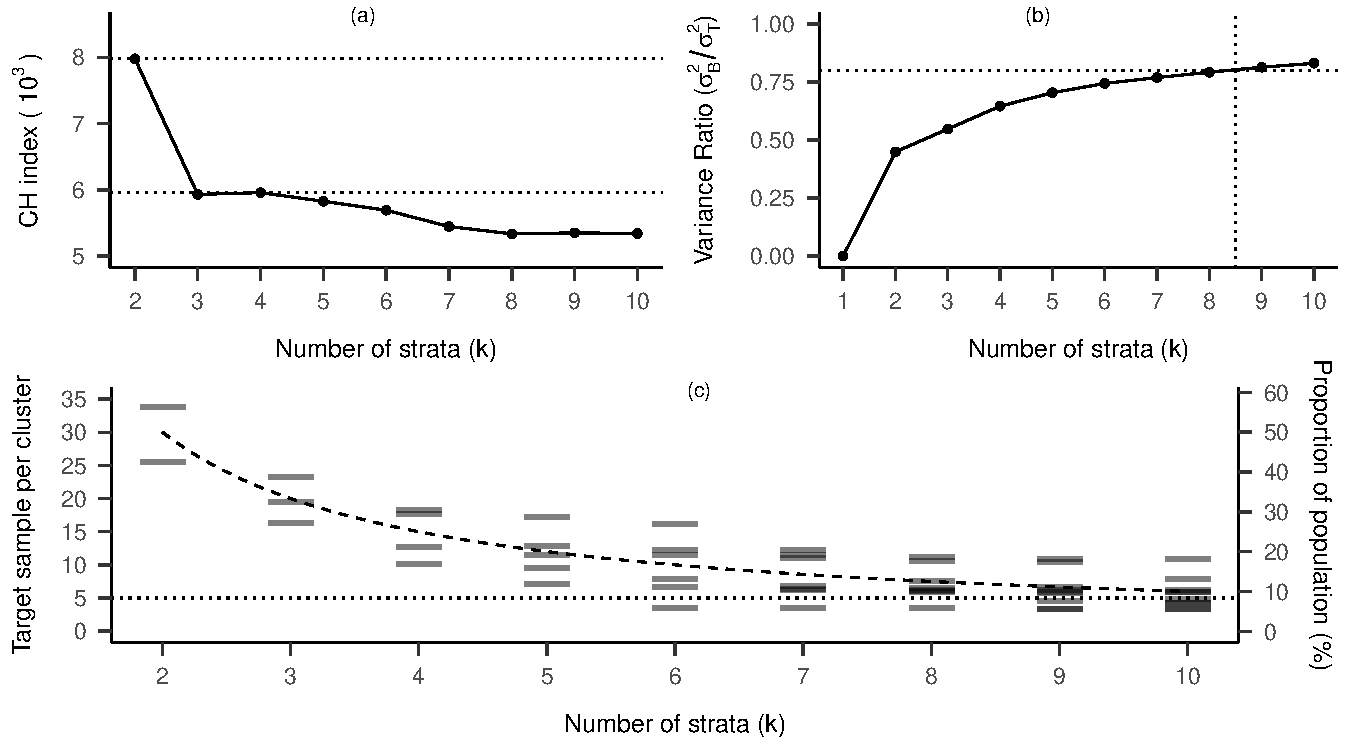
\includegraphics[width=1\linewidth]{6---Paper_files/figure-latex/fig-k-plots-1} \caption{Plots used to determine the number of strata (\(K\)). (a) Calinski-Harabasz index; peaks indicate better fit. (b) Ratio of between-cluster sum of squares to total cluster sum of squares; the horizontal line indicates a cutoff of .8; the vertical line indicates the minimum number of clusters needed to achieve cutoff. (c) Stratum-specific sample size requirements under proportional allocation; the horizontal dotted line indicates a minimum sample size requirement of 5 schools. }\label{fig:fig-k-plots}
\end{figure}

We also considered the proportion of variance that lay between clusters. For each set of \(K = 1,..,10\) total strata, we computed the between- and within-cluster variance for each covariate. We then calculated the proportion of variation that is between strata, denoted \(p_k\), by taking the sum of the between-cluster variances across all covariates, divided by the sum of the between-cluster and within-cluster variances across all covariates.

Figure \ref{fig:fig-k-plots}b plots \(p_k\) against \(K\). The \(K\) for which the rate of change \(p_k\) slows is considered favorable. Tipton (2014b) also recommended selecting the number of clusters such that at least 80\% of the total variation is between clusters; this threshold is indicated in the figure by a horizontal dashed line. In light of this criterion, it seems that at least 9 clusters should be generated. However, we also see that after a sharp initial increase, the slope of the graph begins to level out. This indicates that each additional cluster increases the sampling complexity while explaining less variation in covariates. In practice, the difficulty of sampling may not be worth the small increases in explained variance obtained when using more than 4 or 5 clusters.

Figure \ref{fig:fig-k-plots}c plots the required sample size from each cluster under a proportional allocation. The dashed line indicates the ideal allocation if all clusters were of equal size. We see that cluster sizes become more homogeneous as more clusters are generated. A sensible cutoff may be determined by looking at the size of the smallest cluster. When \(K > 5\), the smallest clusters would require less than 5 sites being sampled, which may be very difficult in practice.

Considering both the statistical criteria and the pragmatic constraints, we generated 5 clusters for purposes of stratification. The strata resulting from this cluster analysis range in size from 1,222 to 2,863 schools. The strata explain 70.43\% of the variation across all covariates (Figure \ref{fig:fig-k-plots}b), with a CH-index of 5,827.31 (Figure \ref{fig:fig-k-plots}a). We also computed variance explained for individual covariates. The proportion of variance explained by the strata differed greatly by covariate, with 5 covariates having between 0 and 11\% variance explained by the strata and 8 variables having from 45\% to 87\% variance explained.\todo[color=blue!20]{Add the proportion of variance for each covariate as a column in Table 1. Reference Table 1 here.}

\hypertarget{B-index}{%
\subsection{\texorpdfstring{\(B\)-index calculations}{B-index calculations}}\label{B-index}}

We used the \(B\)-index as a high-level summary measure of the degree of generalizability of each obtained sample. The index measures the extent of overlap between the distribution of sample selection propensity scores for the obtained sample and for the target population.
Given a set of estimated propensity scores \(\hat\psi_1,...,\hat\psi_N\), we calculated the \(B\) index as
\begin{align}
B = \int_{\hat\psi_{min}-3h_{max}}^{\hat\psi_{max}+3h_{max}}\sqrt{\hat{f}_s(z)\hat{f}_p(z)}dz
\end{align}
where \(\hat\psi_{min}\) and \(\hat\psi_{max}\) are the minimum and maximum values of \(\hat\psi\) respectively, \(\hat{f}_s(z)\) is a Gaussian kernel density estimate of the distribution of propensity scores in the sample, calculated using bandwidth \(h_s\), and \(\hat{f}_p(z)\) is a Gaussian kernel density estimate of the distribution of propensity scores in the non-sampled population, calculated using bandwidth \(h_p\). We calculated the bandwidth \(h\) for the population or sample as follows:
\begin{align}
h = \sigma_{\pi}\left(\frac{4}{3n}\right)^{1/5}
\end{align}
where \(\sigma_{\pi}\) is the standard deviation of the propensity scores.

\hypertarget{SMD-results}{%
\subsection{Standardized Mean Differences}\label{SMD-results}}

Figures \ref{fig:fig-smd-group1}, \ref{fig:fig-smd-group2}, and \ref{fig:fig-smd-group3} display individual covariate balance as measured by standardized mean differences. Each group of plots correspond to the three patterns on performance described in the paper.\todo[color=blue!20]{Add these plots.}







\newpage

\hypertarget{feasibility-results}{%
\subsection{Sampling Feasibility}\label{feasibility-results}}

Figure \ref{fig:fig-rel-per} compares each sampling method to a reference method by plotting the factor of increased difficulty, calculated as the number of schools contacted by comparison method divided by the number of schools contacted by reference method. This gives us another perspective on the relative difficulty of each method. The straight horizontal line represents the reference method.\todo[color=blue!20]{Modify this figure to show the other selection factors too.}\todo[color=blue!20]{Use bubble labels in the plots and remove the figure legend.}



\begin{figure}
\centering
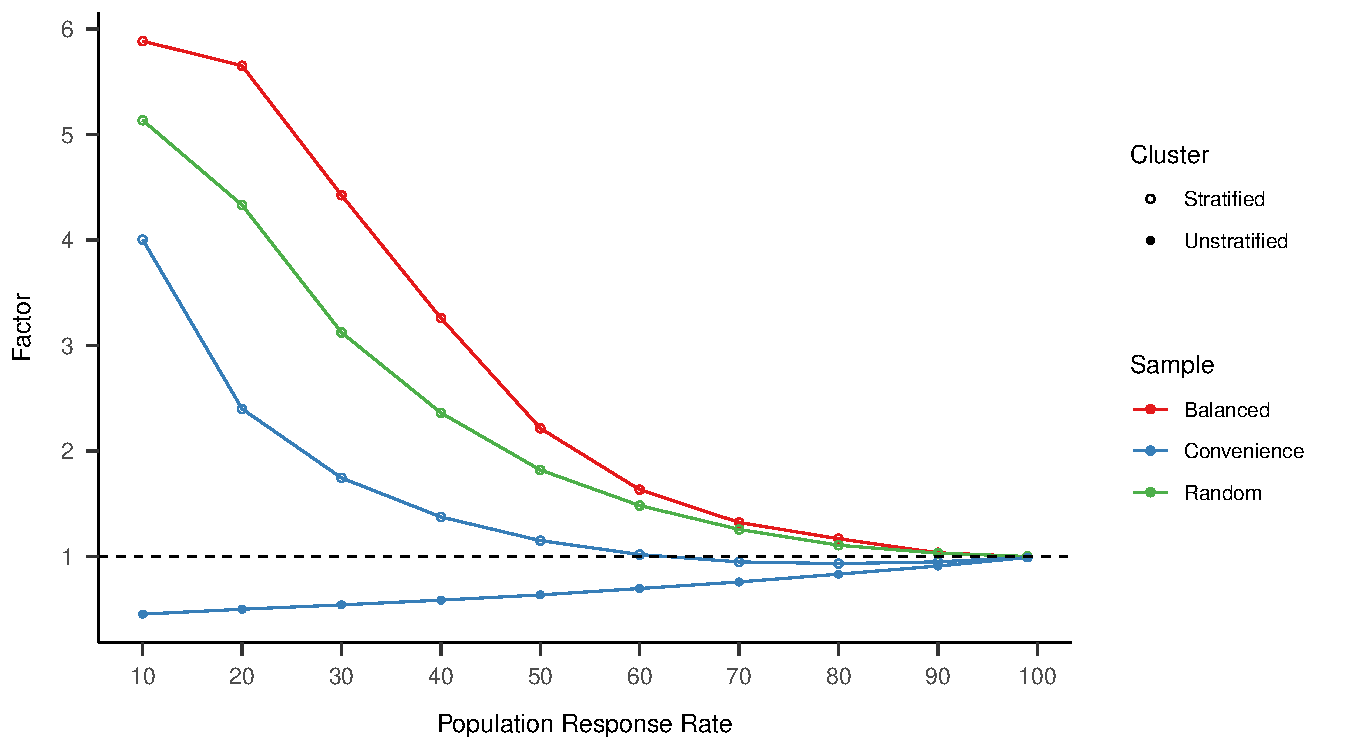
\includegraphics{6---Paper_files/figure-latex/fig-rel-per-1.pdf}
\caption{\label{fig:fig-rel-per}Relative sampling difficulty of each method compared to URS. The the dashed horizontal line indicates equal difficulty (factor of 1).}
\end{figure}

\newpage

\hypertarget{inequity-results}{%
\subsection{Sampling Inequity}\label{inequity-results}}

Figure \ref{fig:fig-gini-curve} displays the Gini curve and coefficient for all sampling methods across participation rates. The index is calculated by computing the area between the diagonal line and the curve. Coefficients of 0 indicate uniform equality across all sampling units, i.e.~all schools have an equal opportunity to be sampled. Coefficients of 1 indicate complete inequality, i.e.~very few schools are constantly being sampled across iterations. Overall, stratification results in lower inequality. However, since balanced sampling prioritizes schools according to set characteristics, the same schools are likely to be sampled each time.\todo[color=blue!20]{This figure is screwed up. The Gini coefficient labels are not in the right place and the lines are so thick that you can't distinguish between stratified and unstratified methods. Please revise or cut this sub-section (and remove reference to it in the main text).}



\begin{sidewaysfigure}[p]
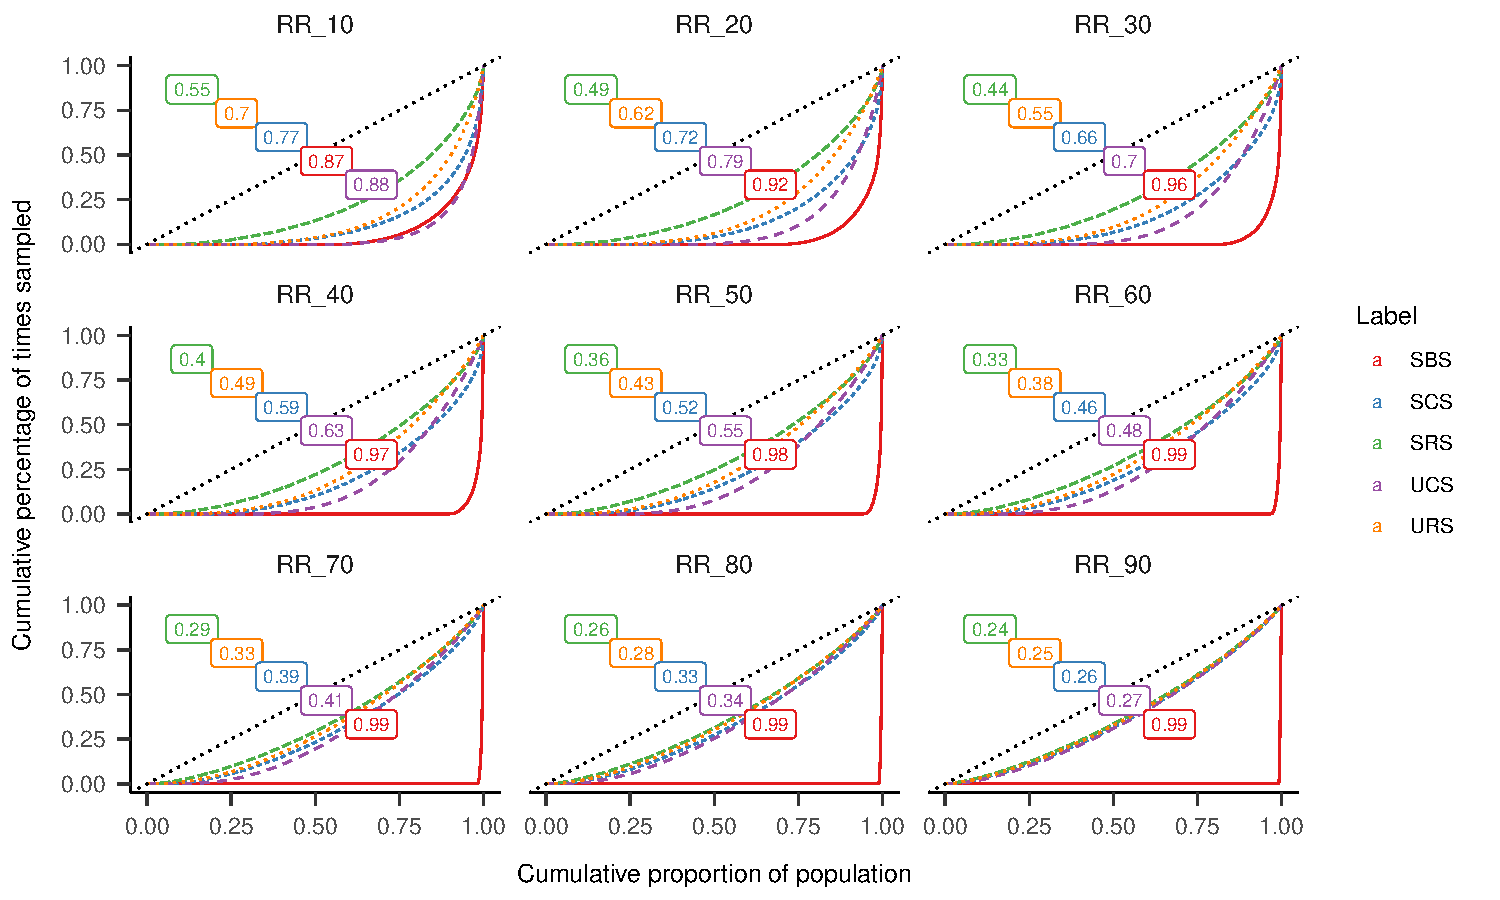
\includegraphics{6---Paper_files/figure-latex/fig-gini-curve-1} \caption{Cumulative probability plot and Gini coefficients representing the inequality of school sampling across sampling methods and population response rates.}\label{fig:fig-gini-curve}
\end{sidewaysfigure}


\end{document}
